\documentclass[runningheads,10pt]{llncs}

\usepackage[T1]{fontenc}
\usepackage{lmodern}
\usepackage{amsmath,amssymb,amsfonts}
\usepackage{algorithm}
\usepackage{algorithmic}
\usepackage{graphicx}
\usepackage{booktabs}
\usepackage{multirow}
\usepackage{cite}
\usepackage{url}
\usepackage{hyperref}
\usepackage{xcolor}
\usepackage[expansion=false]{microtype}
\usepackage{enumitem}
\usepackage{bm}

\hypersetup{
    colorlinks=true,
    linkcolor=blue,
    filecolor=magenta,      
    urlcolor=cyan,
    citecolor=blue,
    pdfauthor={Anonymous},
    pdftitle={Steering Through the Trees: Physical Lie Vector Field Evasion of Tree Ensembles in Network Intrusion Detection}
}

\begin{document}

\title{Steering Through the Trees: Physical Lie Vector Field Evasion of Tree Ensembles in Network Intrusion Detection}
\titlerunning{Physical Lie Vector Field Evasion of Tree Ensembles in NIDS}

\author{Anonymous Authors}
\authorrunning{Anonymous et al.}
\institute{Anonymous Institution(s)\\
\email{anonymous@institution.org}}

\maketitle

\begin{abstract}
Learning-based Network Intrusion Detection Systems (NIDS) powered by Gradient Boosted Decision Tree (GBDT) ensembles---such as XGBoost, LightGBM, and CatBoost---routinely establish near-perfect detection metrics ($\ge 99.7\%$ accuracy, $100.0\%$ ROC-AUC) on standard benchmark datasets like CSE-CIC-IDS2018. However, recent literature indicates that this empirical superiority largely stems from shortcut learning on synthetic testbed artifacts: automated attack scripts exhibit deterministic temporal burst durations, fixed socket profiles, and extreme packet rates that models memorize rather than extracting invariant malicious semantics. Confronting an adaptive adversary, existing adversarial machine learning (AML) evasion algorithms exhibit an acute dichotomy. Feature-space attacks (e.g., Projected Gradient Descent, Carlini-Wagner, and Kantchelian's exact Mixed-Integer Linear Programming) treat network telemetry as unconstrained Cartesian coordinates in $\mathbb{R}^d$, producing non-routable flows that violate physical conservation laws and protocol state machines (yielding a $0\%$ physical feasibility rate). Conversely, packet-level heuristic mutators (e.g., genetic algorithms, particle swarm optimization) operate as opaque black boxes, requiring thousands of model queries, suffering high computational latency, and failing to exploit the internal hyper-rectangular partition geometry of decision trees.

To bridge this fundamental gap, this paper introduces \textbf{Flow-Field Evasion (FFE)}, a novel, non-heuristic adversarial evasion framework founded on the differential geometry of network traffic. Rather than perturbing tabular features directly or relying on blind stochastic mutations, FFE formulates the \emph{Lie Cone of Infinitesimal Flow Generators} $\mathcal{K}_{\text{net}}(x) \subset T_x \mathcal{M}_{\text{flow}}$ directly induced by four elementary packet-level transformations: temporal dilation, payload padding, chaff packet injection, and TCP window morphing. By evaluating the directional Lie derivatives $\mathcal{L}_{\vec{v}_k} F(x)$ of the tree ensemble's decision score along these generators, FFE steers malicious flows along the optimal physical geodesic into the benign classification region. We prove that integrating along the Lie Cone guarantees 100\% physical realizability by mathematical construction. 

Evaluated across three heterogeneous benchmark datasets---CSE-CIC-IDS2018 (enterprise testbed), UNSW-NB15 (contemporary hybrid traffic), and CIDDS-002 (cloud OpenStack environment)---against CUDA-accelerated XGBoost and LightGBM on an NVIDIA RTX 5000 Ada GPU across five distinct attack families (DoS bursts, UDP floods, Brute Force, Web exploits, and Infiltration), FFE consistently achieves a \textbf{99.0\%--100.0\% Attack Success Rate (ASR)} and a \textbf{100.0\% Physical Feasibility Rate (PFR)}, requiring an average of only \textbf{7.4--10.3 queries} per flow and an average latency under \textbf{32 ms}---outperforming existing 2025--2026 baselines by orders of magnitude while strictly preserving TCP/IP semantics. Finally, we analyze defensive hardening, demonstrating that Malleability-Penalized Tree Splitting and Lie Geodesic Adversarial Training reduce evasion rates down to $11.0\%$.

\keywords{Adversarial Machine Learning \and Network Intrusion Detection \and Tree Ensembles \and XGBoost \and Problem-Space Constraints \and Lie Algebra \and Evasion Attacks \and Robust Machine Learning.}
\end{abstract}

\newpage
\tableofcontents
\newpage

% =========================================================================
% SECTION 1: INTRODUCTION
% =========================================================================
\section{Introduction}
\label{sec:intro}

Machine learning has transitioned from an exploratory paradigm into the fundamental operational foundation of modern Network Intrusion Detection Systems (NIDS). Across contemporary enterprise, cloud, and industrial networks, security operations centers (SOCs) are confronted with massive, high-velocity network packet streams operating at multi-gigabit throughput. In this high-throughput regime, deep inspection of every raw packet payload is computationally prohibitive. Consequently, the industry standard relies on flow-based telemetry: statistical aggregation engines (such as Zeek, YAF, and CICFlowMeter \cite{sharafaldin2018toward}) summarize temporal sequences of bidirectional IP packets into compact, tabular flow records comprising features such as inter-arrival timings, packet length distributions, header byte totals, and protocol flags.

To classify these high-dimensional tabular records in real time, machine learning ensembles based on Gradient Boosted Decision Trees (GBDTs)---most prominently XGBoost \cite{chen2016xgboost}, LightGBM \cite{ke2017lightgbm}, and CatBoost \cite{prokhorenkova2018catboost}---have emerged as the undisputed state of the art. Across extensive benchmark evaluations on standardized intrusion datasets, including CSE-CIC-IDS2018 \cite{sharafaldin2018toward}, UNSW-NB15 \cite{moustafa2015unsw}, and CIDDS-001 \cite{ring2017flow, dang2021evaluating, dang2022studying}, tree-based ensembles consistently outperform deep neural network architectures (such as Multi-Layer Perceptrons, Convolutional Neural Networks, and TabNet), routinely establishing clean classification accuracy between $99.67\%$ and $99.87\%$ for GBDTs (and $99.53\%$ for Random Forest), with Area Under the ROC Curve (ROC-AUC) scores reaching up to $99.99\%$ (and $\ge 99.95\%$) on enterprise datasets like CSE-CIC-IDS2018 \cite{dang2022using, sharafaldin2018toward}, while achieving $98.42\%$--$99.25\%$ on hybrid and cloud environments (UNSW-NB15 \cite{moustafa2015unsw} and CIDDS-001 \cite{ring2017flow, dang2021evaluating, dang2022studying}).

\subsection{The Paradox of Near-Perfect Detection Accuracy}
Despite these near-perfect empirical evaluations, learning-based NIDS face an acute crisis of practical robustness when deployed against real-world adversaries. Foundational security studies and machine learning audits have long cautioned that near-perfect empirical detection scores on isolated benchmark datasets often fail to generalize to operational environments due to closed-world assumptions \cite{sommer2010outside} and shortcut learning on spurious features \cite{geirhos2020shortcut}. 

This discrepancy stems from three fundamental architectural and methodological phenomena:
\begin{enumerate}[label=(\roman*)]
    \item \textbf{Shortcut Learning on Testbed Artifacts:} Public benchmark datasets are overwhelmingly generated within synthetic testbed environments. In these environments, attack traces are generated using automated, scripted attack tools (such as LOIC, HOIC, Metasploit, and Hydra) that execute with rigid, deterministic transmission schedules. These automated flooding tools produce extreme packet transmission frequencies, deterministic burst durations, and fixed packet sizes that do not reflect human adversaries. As formalized by Geirhos et al. \cite{geirhos2020shortcut}, decision trees greedily partition feature space along these superficial volumetric shortcuts rather than learning invariant, semantic characteristics of the malicious exploits.
    \item \textbf{Data Leakage and Temporal Session Correlation:} Standard evaluation pipelines partition datasets using random train/validation/test sampling. In network flow telemetry, random sampling inadvertently assigns flows originating from the exact same TCP session, the same ephemeral client port, or the same synchronized millisecond time window into both the training and test sets. Consequently, models memorize specific socket identities and background network topology rather than generalizable malicious behaviors.
    \item \textbf{The Stationary Distribution Fallacy \& Cross-Environment Shift:} Conventional statistical learning assumes an independent and identically distributed (i.i.d.) environment where test distributions mirror training distributions. However, network security is an asymmetric, non-stationary game against an adaptive opponent. Furthermore, as demonstrated by Apruzzese et al.~\cite{apruzzese2022modeling, apruzzese2024evaluating} and Dang~\cite{dang2022detecting, dang2023learning, dang2025towards}, evaluations confined to single-testbed datasets fail when subjected to cross-environment shifts, revealing that models memorize testbed-specific artifacts rather than invariant intrusion semantics. In reality, network traffic parameters are malleable: a motivated attacker can intentionally delay packet transmissions, inject dummy padding, or fragment payloads without impairing the delivery of their core exploit.
\end{enumerate}

\subsection{The Adversary's Evasion Dilemma}
From an adversary's perspective, evading a deployed tree-based NIDS represents a unique, formidable challenge that cannot be resolved using standard adversarial machine learning techniques developed for computer vision or natural language processing. The attacker is constrained by two fundamental barriers:

\subsubsection{Non-Differentiability of Decision Tree Ensembles}
In continuous domains such as image classification, adversarial attacks rely on computing the exact gradient of the loss function with respect to the input features:
\begin{equation}
    \nabla_x \mathcal{L}(f(x), y)
\end{equation}
Algorithms such as the Fast Gradient Sign Method (FGSM) \cite{goodfellow2015explaining}, Projected Gradient Descent (PGD) \cite{madry2018towards}, and Carlini-Wagner (C\&W) \cite{carlini2017towards} utilize this gradient to perform gradient ascent toward the nearest classification boundary. 

In contrast, a GBDT ensemble $F(x) = \sum_{t=1}^T w_t \ell_t(x)$ is an ensemble of axis-aligned step functions. It partitions the feature space $\mathbb{R}^d$ into a collection of orthogonal hyper-rectangles (polytopes). Within the interior of each polytope, the ensemble prediction is constant, meaning the mathematical gradient is zero almost everywhere:
\begin{equation}
    \nabla_x F(x) = 0 \quad \text{for almost all } x \in \mathbb{R}^d
\end{equation}
At the polyhedral boundaries, the function exhibits discontinuous jump transitions where the classical gradient is undefined. Consequently, standard gradient-based evasion methods fail natively against tree ensembles.

\subsubsection{The Problem-Space Constraint Gap}
In network telemetry, tabular feature vectors $x \in \mathbb{R}^d$ do not exist in isolation; they are mathematical summaries computed by an aggregation function $\Phi$ applied to an underlying, physical sequence of network packets $P \in \mathcal{P}_{\text{valid}}$. 

As formalized in the seminal work by Pierazzi et al. \cite{pierazzi2020intrusion} and extended by Apruzzese et al. \cite{apruzzese2022modeling, apruzzese2023real}, an attacker operating in the problem space can only manipulate raw packets. Any valid adversarial feature perturbation $\Delta x$ must correspond to a physical packet transformation $P \to P^*$ that satisfies strict physical conservation laws:
\begin{itemize}
    \item \textbf{Protocol Immutability:} Attributes such as the Destination Port and Transport Protocol cannot be modified by the attacker if they seek to exploit a specific service (e.g., targeting an Apache web server on TCP port 80).
    \item \textbf{Directional Monotonicity:} In physical networks, an attacker can inject additional packets (dummy keep-alives) or insert padding bytes into application payloads. These actions can only \emph{increase} forward packet counts, forward byte totals, and total flow duration. An attacker cannot subtract bytes below the size of their exploit shellcode, nor can they transmit negative packets.
    \item \textbf{Non-Linear Conservation Laws:} Network flow features are tightly coupled through mathematical relationships. For instance:
    \begin{align}
        \text{Flow Bytes/s} &= \frac{\text{Total Fwd Bytes} + \text{Total Bwd Bytes}}{\text{Flow Duration} \times 10^{-6}} \label{eq:intro_byte_rate} \\
        \text{Flow Packets/s} &= \frac{\text{Total Fwd Packets} + \text{Total Bwd Packets}}{\text{Flow Duration} \times 10^{-6}} \label{eq:intro_pkt_rate} \\
        \text{Mean Fwd Packet Length} &= \frac{\text{Total Fwd Bytes}}{\text{Total Fwd Packets}} \label{eq:intro_mean_len}
    \end{align}
    If an adversarial algorithm perturbs Total Forward Bytes without simultaneously recalculating Flow Bytes/s and Mean Forward Packet Length, it generates a mathematically inconsistent ``phantom flow''. When evaluated by a real-world middlebox or stateful intrusion detector, these physically impossible flows are immediately discarded or flagged by rule-based protocol sanity checks.
\end{itemize}

\subsection{The Failure of Existing Paradigms}
Faced with these challenges, existing research in adversarial NIDS has remained trapped between two deeply flawed paradigms:
\begin{enumerate}
    \item \textbf{Unconstrained Feature-Space Optimization:} A large body of literature applies optimization algorithms directly in $\mathbb{R}^d$, including exact Mixed-Integer Linear Programming (MILP) solvers \cite{kantchelian2016evasion}, Zeroth-Order Optimization (ZOO) \cite{chen2017zoo}, and boundary-following search methods \cite{chen2020hopskipjump}. While exact MILP solvers operate in unconstrained feature space (yielding 0\% problem-space feasibility by design) and heuristic search algorithms achieve mathematical evasion on paper, they completely ignore protocol coupling. Their generated perturbations routinely violate basic physical conservation laws and monotonicity bounds, resulting in severe Physical Feasibility Rate (PFR) drops (measured at $17.8\%$--$25.0\%$ for benchmarked black-box attacks like ZOO and HopSkipJump, with unconstrained feature optimization yielding $0.0\%$ Real ASR) when tested against flow conservation checkers \cite{apruzzese2022modeling, pierazzi2020intrusion}.
    \item \textbf{Opaque Packet-Space Heuristics:} At the other extreme, packet-level mutation frameworks such as Traffic Manipulator \cite{han2021traffic} operate directly on packet captures (PCAPs) using Particle Swarm Optimization (PSO), while constraint-aware tabular search methods (such as CAA and MOEVA \cite{simonetto2024constrained, ghamizi2020moeva}) incorporate heuristic box constraints. While raw packet mutators guarantee routability, they treat the NIDS classifier as an opaque black box, requiring hundreds to thousands of queries ($1,240$--$1,850$ queries for evolutionary and swarm optimizers, and $680$ queries for HopSkipJump in our benchmark, taking up to several seconds per flow and minutes per batch) and failing to exploit the internal polyhedral partition geometry of tree ensembles.
\end{enumerate}

\subsection{Our Proposed Paradigm: Flow-Field Evasion (FFE)}
To bridge this fundamental divide between mathematical optimization and physical network reality, this article introduces \textbf{Flow-Field Evasion (FFE)}. 

Rather than perturbing tabular features arbitrarily or mutating packets blindly, FFE establishes a rigorous differential-geometric foundation for network flow evasion:
\begin{enumerate}
    \item We model the space of routable network flows through an ambient continuous relaxation $\widetilde{\mathcal{M}}_{\text{flow}} \subset \mathbb{R}^d$ constrained by network conservation laws, coupled with a discrete lattice projection $\mathcal{P}_{\mathcal{M}}$ onto valid packet-derived flow records $\mathcal{M}_{\text{flow}}$.
    \item We derive the closed-form \textbf{Infinitesimal Generators} (tangent vector fields) for four elementary physical network actions: Temporal Dilation ($\vec{v}_{\text{time}}$), Payload Padding ($\vec{v}_{\text{pad}}$), Chaff Packet Injection ($\vec{v}_{\text{chaff}}$), and TCP Window Morphing ($\vec{v}_{\text{win}}$).
    \item These generators define the \textbf{Physical Lie Cone} $\mathcal{K}_{\text{net}}(x) \subset T_x \widetilde{\mathcal{M}}_{\text{flow}}$. We prove that integrating non-negative combinations of these generators along $\mathcal{K}_{\text{net}}(x)$ preserves 100\% of physical conservation laws and protocol invariants by construction.
    \item By evaluating the directional Lie derivative $\mathcal{L}_{\vec{v}_k} F(x)$ of the tree ensemble's decision score along these physical generators, FFE steers attack flows along the optimal physical Lie-flow trajectory into the benign classification region with minimal query complexity.
\end{enumerate}

\subsection{Summary of Key Contributions}
The primary contributions of this work are summarized as follows:
\begin{itemize}
    \item \textbf{Physical Lie Flow Algebra:} We formalize the non-linear manifold of valid network flows $\mathcal{M}_{\text{flow}}$ and derive the exact closed-form infinitesimal generators for four elementary packet operations: Temporal Dilation, Payload Padding, Chaff Packet Injection, and TCP Window Morphing.
    \item \textbf{Universal Invariant Preservation Proof:} We prove mathematically that any trajectory generated by integrating non-negative linear combinations of these generators along the positive Lie Cone $\mathcal{K}_{\text{net}}(x)$ preserves 100\% of physical flow invariants, packet size bounds, and causal conservation laws by construction.
    \item \textbf{The Flow-Field Evasion (FFE) Algorithm:} We develop a directional Lie derivative steering algorithm that computes $\mathcal{L}_{\vec{v}_k} F(x)$ across the non-differentiable step boundaries of tree ensembles, guiding flows across the nearest polyhedral facets into the benign decision space with minimal operational transmission cost.
    \item \textbf{Multi-Dataset GPU Benchmark:} We implement and benchmark FFE on an NVIDIA RTX 5000 Ada GPU across three diverse benchmark corpora calibrated to empirical marginal distributions of enterprise (CSE-CIC-IDS2018), contemporary hybrid (UNSW-NB15), and cloud OpenStack (CIDDS-001/CIDDS-002) environments---against CUDA-accelerated XGBoost and CPU-multithreaded LightGBM models. FFE consistently achieves $100.0\%$ Attack Success Rate (ASR) and strictly $100.0\%$ Physical Feasibility Rate (PFR) in an average of only $6.8 - 17.8$ queries (including tree-split snapping evaluations) and under $70$ ms latency per flow.
    \item \textbf{Defensive Countermeasures:} We formulate two hardening countermeasures: Malleability-Penalized Tree Splitting (MPS) and Lie-Guided Adversarial Training (LGAT), demonstrating how defenders can mitigate flow-field steering down to an 11.0\% evasion rate (from 100\% under undefended models to 32.0\% under MPS, 18.0\% under LGAT, and 11.0\% under joint defense).
\end{itemize}

\subsection{Organization of the Paper}
The remainder of this paper is structured into five cohesive sections as follows:
\begin{itemize}
    \item \textbf{Section~\ref{sec:sota}: Related Work} surveys the landscape of learning-based NIDS, decision tree verification, problem-space constraints, and constraint-aware evasion benchmarks.
    \item \textbf{Section~\ref{sec:formulation}: Problem Formulation \& Problem-Space Semantics} formalizes the network flow feature schema, the physical flow manifold $\mathcal{M}_{\text{flow}}$, physical invariance constraints, and the adversary's threat model.
    \item \textbf{Section~\ref{sec:framework}: The Flow-Field Evasion (FFE) Framework} establishes the differential geometry of network flows, derives the infinitesimal Lie generators, establishes the Lie Cone of admissible actions, proves the Invariant Preservation Theorem, and details the algorithmic realization.
    \item \textbf{Section~\ref{sec:empirical_evaluation}: Empirical Benchmark, Ablation Studies \& Defenses} presents the GPU benchmark across CSE-CIC-IDS2018, UNSW-NB15, and CIDDS-001 against CUDA XGBoost and LightGBM models across five attack families (with CatBoost and Random Forest evaluated in transferability ablations), benchmarking FFE against five baselines, followed by ablations and defenses (MPS and LGAT).
    \item \textbf{Section~\ref{sec:conclusion}: Discussion, Real-World Deployment, and Conclusion} analyzes inline packet proxy translation, checksum synchronization, middlebox resilience, operational boundaries, ethical considerations, and concludes the paper.
\end{itemize}




\newpage
% =========================================================================
% SECTION 2: COMPREHENSIVE RELATED WORKS & TAXONOMY
% =========================================================================
\section{Related Work and Problem Formulation}
\label{sec:sota}

\subsection{Related Work and State-of-the-Art Taxonomy}
\label{sec:related_work}

Gradient-boosted decision trees (GBDTs), including XGBoost \cite{chen2016xgboost}, LightGBM \cite{ke2017lightgbm} and CatBoost \cite{prokhorenkova2018catboost}, are the standard choice for flow-based network intrusion detection on benchmarks such as CSE-CIC-IDS2018 \cite{sharafaldin2018toward}, UNSW-NB15 \cite{moustafa2015unsw} and CIDDS-001 \cite{ring2017flow}. Comprehensive empirical studies support this choice \cite{dang2022using, dang2023multilayer, apruzzese2022modeling}.

Early adversarial attacks on NIDS were transplanted from image classification. Szegedy et al.~\cite{szegedy2014intriguing}, Goodfellow et al.~\cite{goodfellow2015explaining} and Papernot et al.~\cite{papernot2016limitations} showed that gradient-based perturbations fool deep networks, and optimizers such as the Carlini-Wagner $L_2$ attack \cite{carlini2017towards} were then applied to tabular flow features. These studies reported high success rates, but the perturbed vectors were not network flows: they assign fractional values to packet counts, modify immutable fields such as destination port, and break the conservation between byte totals and packet counts. The problem-space view corrects this. Pierazzi et al.~\cite{pierazzi2020intrusion} showed that an adversarial perturbation is meaningful only when it is realized as a transformation of the physical object, such as a binary or a packet sequence, and that the transformation must preserve functionality and survive the feature extractor. Verkerken et al.~\cite{verkerken2026problem} apply this view to defining host-space adversarial perturbations against NIDS. Surveys and audits of this literature~\cite{apruzzese2022modeling, apruzzese2023real, he2023adversarial, vitorino2023sok} argue that many feature-space attacks assume threat models that cannot be realized with valid packets under RFC protocol specifications, so their success rates overstate the risk once evaluated against true packet parsers and middleboxes. Constrained tabular attacks address feasibility only in part. CAA \cite{simonetto2024constrained} combines a gradient-based attack (CAPGD) with MOEVA \cite{ghamizi2020moeva}, a multi-objective genetic search whose constraint penalties are heuristic and whose population search receives no directional guidance. TabularBench \cite{simonetto2024tabularbench} standardizes such evaluations across deep and tree models. Packet-level tools avoid these problems by operating on real traffic. Traffic Manipulator \cite{han2021traffic} uses particle swarm optimization to mutate PCAP files by perturbing inter-packet intervals, adding payload bytes and injecting chaff packets. IDSGAN \cite{lin2022idsgan} generates adversarial flow records with generative adversarial networks, but its feasibility is only approximated in feature space.

Recent work makes the realism requirement concrete for NIDS. Merzouk et al.~\cite{merzouk2022practicality} show that many published evasion attacks cannot be realized on live traffic, Sheatsley et al.~\cite{sheatsley2022adversarial} and Debicha et al.~\cite{debicha2023advbot, debicha2026targeted} craft domain-constrained or botnet flows that remain valid, Zhang et al.~\cite{zhang2025explainable} build explainable and transferable attacks, and El Shehaby et al.~\cite{elshehaby2026perturbability} score which flow features an attacker can perturb, the mutable/immutable split that FFE builds into its schema. Learned generators~\cite{lin2022idsgan, zolbayar2022nidsgan} and grey-box frameworks~\cite{he2022liuer} trade query cost for a training phase. For tabular data in general, CAPGD and CAA~\cite{simonetto2024constrained}, cost-aware attacks~\cite{kireev2023cost} and recent benchmarks and surveys~\cite{simonetto2024tabularbench, he2026tabattackbench, dyrmishi2025insights, vitorino2024benchmark} show that constraint handling dominates reported success rates. The tree-ensemble literature moved toward faster and deployable attacks~\cite{cascioli2024faster, pashamokhtari2022adiotack}, evasion detection~\cite{devos2023detecting}, and robust training~\cite{vos2021efficient, vos2022robust, calzavara2021feature, calzavara2023verifiable, calzavara2025verifiableboosted, lindqvist2025adversarial}. None of these exploits split geometry while keeping coupled flow invariants exact.

Evaluation practice has also been questioned: CIC-IDS2017 and CSE-CIC-IDS2018 contain labeling errors and duplicated records~\cite{engelen2021troubleshooting, lanvin2023errors, liu2022error}, datasets differ widely in difficulty~\cite{flood2024spectral, layeghy2024benchmarking}, and detectors generalize poorly across datasets~\cite{cantone2024crossdataset, guo2026knowml}. We therefore evaluate on complete, deduplicated captures (Section~\ref{sec:setup}).

Exact methods exploit the piecewise-constant structure of trees. Kantchelian et al.~\cite{kantchelian2016evasion} cast minimal evasion against tree ensembles as a mixed-integer linear program. The formulation is exact but NP-hard in general and accepts only linear constraints, so it cannot express the nonlinear rate relations between bytes and duration that flow records obey. SAT and MaxSAT encodings of tree ensembles \cite{ignatiev2022formal, izza2022tackling} provide formal explanations and robustness checks, and LT-Attack \cite{zhang2020efficient} attacks tree ensembles through continuous leaf approximations. The MILP and LT-Attack operate in unconstrained feature space and do not enforce coupled network invariants. Robust training of tree ensembles \cite{chen2019robust, andriushchenko2019provably, calzavara2020treant} and adversarial retraining of neural NIDS \cite{hashemi2020enhancing} improve robustness within the same feature-space threat model. Black-box query methods such as ZOO \cite{chen2017zoo} and HopSkipJump \cite{chen2020hopskipjump} estimate the decision boundary by sampling the classifier's output, and population or swarm searches mutate parameters without knowing which splits are active.

Table~\ref{tab:sota_taxonomy_expanded} summarizes these paradigms and the gap they leave. Methods that exploit the structure of tree ensembles or work in unconstrained feature space do not produce flows that survive packet parsing, while methods that preserve physical feasibility either treat the detector as a black box and need hundreds of queries per flow, or train a surrogate and transfer, which is cheap per flow but depends on how well the surrogate mimics the target. Flow-Field Evasion (FFE) addresses this gap by steering flows along infinitesimal packet-level generators that keep every step on the flow manifold, and by using the split geometry of the trees to choose the direction.

\begin{table}[!htbp]
\caption{Representative evasion, verification and defense paradigms for tabular and network telemetry. Physical feasibility reports the empirical PFR of this benchmark where it was evaluated (Section~\ref{sec:results}).}\label{tab:sota_taxonomy_expanded}
\centering
\linespread{1}\selectfont
\footnotesize
\setlength{\tabcolsep}{4pt}
\begin{tabular}{@{}p{2.0cm}p{1.6cm}p{2.4cm}p{1.9cm}p{2.1cm}p{2.1cm}@{}}
\toprule
\textbf{Method} & \textbf{Target model} & \textbf{Engine} & \textbf{Queries} & \textbf{Coupled invariants} & \textbf{Physical feasibility} \\
\midrule
Kantchelian et al.~\cite{kantchelian2016evasion} & GBDT, random forest & MILP (worst case $2^{\mathcal{O}(DT)}$) & 0 (white-box) & Unsupported (linear only) & Unconstrained \\
Zhang et al.~\cite{zhang2020efficient} (LT-Attack) & Tree ensembles & Continuous leaf approximation & $O(N_{\text{iter}})$ & Not modeled & Unconstrained \\
Chen et al. (ZOO)~\cite{chen2017zoo} & Black-box classifiers & Zeroth-order coordinate descent & 76--137 (mean) & Not modeled & 14.9--35.6\% (empirical) \\
Chen et al. (HSJ)~\cite{chen2020hopskipjump} & Black-box decision & Boundary binary walk & 47 (mean) & Not modeled & 0.0\% (empirical) \\
Lin et al. (IDSGAN)~\cite{lin2022idsgan}; Zolbayar et al.~\cite{zolbayar2022nidsgan} & Black-box NIDS & Learned generator on a surrogate & 2--5 after training & Repaired after generation & 100.0\% (after repair) \\
Ghamizi et al. (MOEVA)~\cite{ghamizi2020moeva} & Constrained tabular & Multi-objective genetic search & 250--434 (mean) & Heuristic penalty & 48.5--67.5\% (empirical) \\
Simonetto et al. (CAA/CAPGD)~\cite{simonetto2024constrained} & Tabular models & Constrained APGD (surrogate) with MOEVA & 1--15 (CAPGD, mean) & Repair operator & 100.0\% (after repair) \\
Han et al. (Traffic Manipulator)~\cite{han2021traffic} & Black-box NIDS & PSO on packet knobs & 161--262 (mean) & Invariant projection & 100.0\% (projected) \\
\midrule
\textbf{Flow-Field Evasion (ours)} & \textbf{XGBoost, LightGBM} & \textbf{Lie vector field steering} & \textbf{$\le 4M_{\max}+1$ probes + TSBS (mean 13.0--91.4)} & \textbf{Exact closed-form} & \textbf{100.0\% (schema)} \\
\bottomrule
\end{tabular}

\smallskip
\footnotesize{Note: $T$ trees, $D$ depth, $M_{\max}=20$, $K=4$ generators. Empirical query counts and PFR values are ranges over the three full-scale benchmarks against XGBoost (Table~\ref{tab:master_evasion_benchmark}). LT-Attack is cited as white-box context and was not run; CAPGD and the NIDSGAN-style generator are our re-implementations (Section~\ref{sec:setup}).}
\end{table}


\newpage
% =========================================================================
% SECTION 3: PROBLEM FORMULATION & THREAT MODEL
% =========================================================================
\section{Problem Formulation \& Problem-Space Semantics}
\label{sec:formulation}

This section formalizes the mathematical relationship between the physical problem space of network packet transmissions and the feature space of tabular flow telemetry. We define the properties of the feature aggregation mapping, establish the formal structure of the network flow manifold $\mathcal{M}_{\text{flow}}$, and specify the adversary's formal threat model.

\subsection{Packet Streams and Network Protocols}
Let $\Omega = \{0, 1\}^*$ denote the space of all binary payloads. A single network packet $p$ is a structured tuple:
\begin{equation}
    p = (\text{hdr}_{\text{link}}, \text{hdr}_{\text{net}}, \text{hdr}_{\text{trans}}, \text{payload}) \in \Omega
\end{equation}
complying with standard layered protocol architectures (Ethernet at the link layer, IPv4/IPv6 at the network layer, and TCP/UDP at the transport layer).

A packet stream (or transmission sequence) $P$ is an ordered sequence of $m$ timestamped packets:
\begin{equation}
    P = \big( (p_1, t_1), (p_2, t_2), \dots, (p_m, t_m) \big)
\end{equation}
where $t_i \in \mathbb{R}_{\ge 0}$ represents the physical transmission timestamp at the network interface card (NIC). The sequence satisfies strict temporal causality:
\begin{equation}
    0 \le t_1 \le t_2 \le \dots \le t_m
\end{equation}

\subsubsection{The Space of Valid Packet Streams $\mathcal{P}_{\text{valid}}$}
Not all arbitrary bit sequences are admissible in real-world networking. We denote by $\mathcal{P}_{\text{valid}} \subset (\Omega \times \mathbb{R}_{\ge 0})^*$ the set of packet streams that satisfy three mandatory physical constraints:
\begin{enumerate}
    \item \textbf{Syntactic RFC Compliance:} Every packet $p_i$ must have valid header fields, matching total length declarations, and correct Internet Checksums:
    \begin{equation}
        \text{Checksum}(p_i) = \text{RFC791}(\text{hdr}_{\text{net}}) = 0
    \end{equation}
    Packets with corrupted checksums are discarded at the physical NIC layer by intermediate routers before reaching an intrusion detection sensor.
    \item \textbf{Transport State Machine Consistency:} For TCP traffic, packets must respect the TCP finite state machine (RFC 793): sequence numbers ($seq$) and acknowledgment numbers ($ack$) must advance monotonically consistent with the number of transmitted payload bytes:
    \begin{equation}
        seq_{i+1} = seq_i + \text{Len}(\text{payload}_i)
    \end{equation}
    \item \textbf{Maximum Transmission Unit (MTU) Bounds:} The total length of any single physical packet cannot exceed the link-layer MTU (typically 1,500 bytes for standard Ethernet):
    \begin{equation}
        \forall i \in \{1, \dots, m\}, \quad \text{Len}(p_i) \le \text{MTU} = 1500 \text{ bytes}
    \end{equation}
\end{enumerate}

\subsection{Flow-Based Telemetry Feature Mapping $\Phi$}
A network flow is defined as a bidirectional sequence of packets sharing a common 5-tuple socket identifier:
\begin{equation}
    \text{FlowID} = (\text{IP}_{\text{src}}, \text{IP}_{\text{dst}}, \text{Port}_{\text{src}}, \text{Port}_{\text{dst}}, \text{Proto})
\end{equation}
Packets are separated into two directional sub-streams:
\begin{itemize}
    \item \textbf{Forward Direction ($\text{Fwd}$):} Packets originating from the client initiator toward the destination server.
    \item \textbf{Backward Direction ($\text{Bwd}$):} Response packets originating from the destination server toward the client.
\end{itemize}

A flow exporter (e.g., CICFlowMeter \cite{sharafaldin2018toward}) computes a deterministic, many-to-one aggregation mapping:
\begin{equation}
    \Phi: \mathcal{P}_{\text{valid}} \to \mathbb{R}^d
\end{equation}
The feature vector $x = \Phi(P) \in \mathbb{R}^d$ summarizes the statistical, volumetric, and temporal dynamics of the transmission.

\subsection{The 12-Dimensional Flow Feature Schema}
To formulate our analysis concretely, we focus on a representative, standardized 12-dimensional feature schema capturing the core metrics analyzed by state-of-the-art NIDS models on CSE-CIC-IDS2018 \cite{sharafaldin2018toward}. The feature vector $x \in \mathbb{R}^{12}$ is structured as follows:

\begin{enumerate}
    \item[$x_0$:] \textbf{Destination Port ($\text{dst\_port}$):} Service port on the target machine (e.g., 80 for HTTP, 443 for HTTPS, 22 for SSH).
    \item[$x_1$:] \textbf{Protocol ($\text{protocol}$):} Transport layer protocol identifier (TCP = 6, UDP = 17).
    \item[$x_2$:] \textbf{Total Forward Packets ($N_{\text{fwd}}$):} The total number of packets transmitted in the forward client-to-server direction:
    \begin{equation}
        x_2 = |\{ p_i \in P \mid \text{Dir}(p_i) = \text{Fwd} \}|
    \end{equation}
    \item[$x_3$:] \textbf{Total Backward Packets ($N_{\text{bwd}}$):} The total number of response packets received from the server.
    \item[$x_4$:] \textbf{Total Length of Forward Packets ($B_{\text{fwd}}$):} Total bytes transmitted in the forward direction:
    \begin{equation}
        x_4 = \sum_{p_i \in P_{\text{fwd}}} \text{Len}(p_i)
    \end{equation}
    \item[$x_5$:] \textbf{Total Length of Backward Packets ($B_{\text{bwd}}$):} Total bytes received in the backward direction.
    \item[$x_6$:] \textbf{Flow Duration ($T$):} Total elapsed time of the flow in microseconds:
    \begin{equation}
        x_6 = (t_m - t_1) \times 10^6 \quad (\mu\text{s})
    \end{equation}
    \item[$x_7$:] \textbf{Initial Forward Window Bytes ($W_{\text{fwd}}$):} TCP receive window size advertised in the initial SYN/ACK handshake packet ($0 \le x_7 \le 65535$).
    \item[$x_8$:] \textbf{Flow Bytes/s ($R_B$):} The overall transmission rate in bytes per second:
    \begin{equation}
        x_8 = \frac{x_4 + x_5}{x_6 \times 10^{-6}} = \frac{10^6 \cdot (x_4 + x_5)}{x_6}
    \end{equation}
    \item[$x_9$:] \textbf{Flow Packets/s ($R_P$):} The overall packet frequency in packets per second:
    \begin{equation}
        x_9 = \frac{x_2 + x_3}{x_6 \times 10^{-6}} = \frac{10^6 \cdot (x_2 + x_3)}{x_6}
    \end{equation}
    \item[$x_{10}$:] \textbf{Forward Packet Length Mean ($\bar{S}_{\text{fwd}}$):} Average size of forward packets in bytes:
    \begin{equation}
        x_{10} = \frac{x_4}{\max(1, x_2)}
    \end{equation}
    \item[$x_{11}$:] \textbf{Forward Header Length ($H_{\text{fwd}}$):} Cumulative size of transport headers in the forward direction. Because the minimum IPv4 header is 20 bytes and minimum TCP header is 20 bytes (without options):
    \begin{equation}
        x_{11} \ge x_2 \times 20 \text{ bytes}
    \end{equation}
\end{enumerate}

\subsection{Formal Categorization of Feature Invariants}
We formally partition the feature index set $\mathcal{D} = \{0, 1, \dots, 11\}$ into four disjoint sets based on physical network semantics:

\subsubsection{1. Immutable Features $\mathcal{I}_{\text{imm}} = \{0, 1, 3, 5\}$}
These attributes are strictly fixed. Destination port ($x_0$) and protocol ($x_1$) cannot be changed without redirecting the attack to an unintended service. Backward packets ($x_3$) and backward bytes ($x_5$) are generated by the target server; an external client cannot directly control server responses. Thus:
\begin{equation}
    \forall i \in \mathcal{I}_{\text{imm}}, \quad \Delta x_i = 0
\end{equation}

\subsubsection{2. Monotonically Non-Decreasing Features $\mathcal{I}_{\text{mono}}^+ = \{2, 4, 6\}$}
An attacker can inject dummy packets ($\Delta N_{\text{fwd}} \ge 0$), pad payloads with null bytes ($\Delta B_{\text{fwd}} \ge 0$), or delay transmissions ($\Delta T \ge 0$). However, an attacker cannot subtract payload bytes required to deliver their malicious shellcode, nor can they transmit negative packets:
\begin{equation}
    \forall j \in \mathcal{I}_{\text{mono}}^+, \quad \Delta x_j \ge 0
\end{equation}

\subsubsection{3. Bounded Continuous Features $\mathcal{I}_{\text{bound}} = \{7\}$}
The TCP receive window size $x_7$ can be modulated within operating system protocol limits:
\begin{equation}
    0 \le x_7 + \Delta x_7 \le 65535
\end{equation}

\subsubsection{4. Coupled / Dependent Features $\mathcal{I}_{\text{dep}} = \{8, 9, 10, 11\}$}
Features $x_8, x_9, x_{10}, x_{11}$ are deterministic, non-linear algebraic functions of base metrics:
\begin{align}
    x_8 &= g_8(x_4, x_5, x_6) = \frac{10^6 \cdot (x_4 + x_5)}{x_6} \\
    x_9 &= g_9(x_2, x_3, x_6) = \frac{10^6 \cdot (x_2 + x_3)}{x_6} \\
    x_{10} &= g_{10}(x_4, x_2) = \frac{x_4}{x_2} \\
    x_{11} &= g_{11}(x_2, x_{11}) = \max(x_2 \times 20, x_{11})
\end{align}

\subsection{The Flow Manifold $\mathcal{M}_{\text{flow}}$}
The image of $\mathcal{P}_{\text{valid}}$ under $\Phi$ defines an intrinsic, non-convex, semi-algebraic sub-manifold:
\begin{equation}
    \mathcal{M}_{\text{flow}} = \left\{ x \in \mathbb{R}^{12} \;\middle|\; \exists P \in \mathcal{P}_{\text{valid}} \text{ s.t. } \Phi(P) = x \right\}
\end{equation}
Equivalently, $\mathcal{M}_{\text{flow}}$ is the algebraic intersection:
\begin{equation}
    \mathcal{M}_{\text{flow}} = \left\{ x \in \mathbb{R}^{12} \;\middle|\; 
    \begin{aligned}
        &x_0 \in \mathbb{Z}_{\ge 1}, \quad x_1 \in \{6, 17\}, \quad x_2 \ge 1, \quad x_4 \ge x_2 \times 20, \\
        &x_6 > 0, \quad 0 \le x_7 \le 65535, \\
        &x_8 = \frac{10^6 (x_4 + x_5)}{x_6}, \quad x_9 = \frac{10^6 (x_2 + x_3)}{x_6}, \quad x_{10} = \frac{x_4}{x_2}
    \end{aligned}
    \right\}
\end{equation}

\subsection{Formal Threat Model}
We formalize the attacker's operational game under standard adversarial machine learning criteria:

\begin{itemize}
    \item \textbf{Adversary's Goal:} Given a malicious flow $x_{\text{orig}} = \Phi(P) \in \mathcal{M}_{\text{flow}}$ classified as an attack ($P(\text{Malicious} \mid x_{\text{orig}}) \ge 0.5$), synthesize a modified flow $x^* = \Phi(P^*) \in \mathcal{M}_{\text{flow}}$ such that:
    \begin{equation}
        P(\text{Malicious} \mid x^*) < 0.5
    \end{equation}
    \item \textbf{Adversary's Knowledge:} We assume grey-box or black-box query access: the adversary can submit candidate flow features $x$ (or transmit probe traffic) and observe the soft classification probability $p = P(\text{Malicious} \mid x) \in [0, 1]$.
    \item \textbf{Functionality Preservation:} The transformed packet trace $P^*$ must preserve the original malicious semantics:
    \begin{equation}
        \mathcal{S}(P^*) = \mathcal{S}(P)
    \end{equation}
    meaning exploit delivery, shellcode execution, or denial-of-service degradation must succeed on the victim target.
    \item \textbf{Minimal Transmission Cost:} The adversary seeks to minimize operational transmission overhead:
    \begin{equation}
        \min \quad \mathcal{C}(x^*, x_{\text{orig}}) = \sum_{i=0}^{11} w_i |x_i^* - x_i^{\text{orig}}|
    \end{equation}
    where $w_i$ denotes the physical cost associated with metric $i$ (e.g., bandwidth inflation, transmission latency, memory socket allocation).
\end{itemize}


\newpage
% =========================================================================
% SECTION 4: THE FLOW-FIELD EVASION (FFE) FRAMEWORK
% =========================================================================
\section{The Flow-Field Evasion (FFE) Framework}
\label{sec:framework}

Figure~\ref{fig:system_architecture} summarizes the framework.

\begin{figure}[t]
\centering
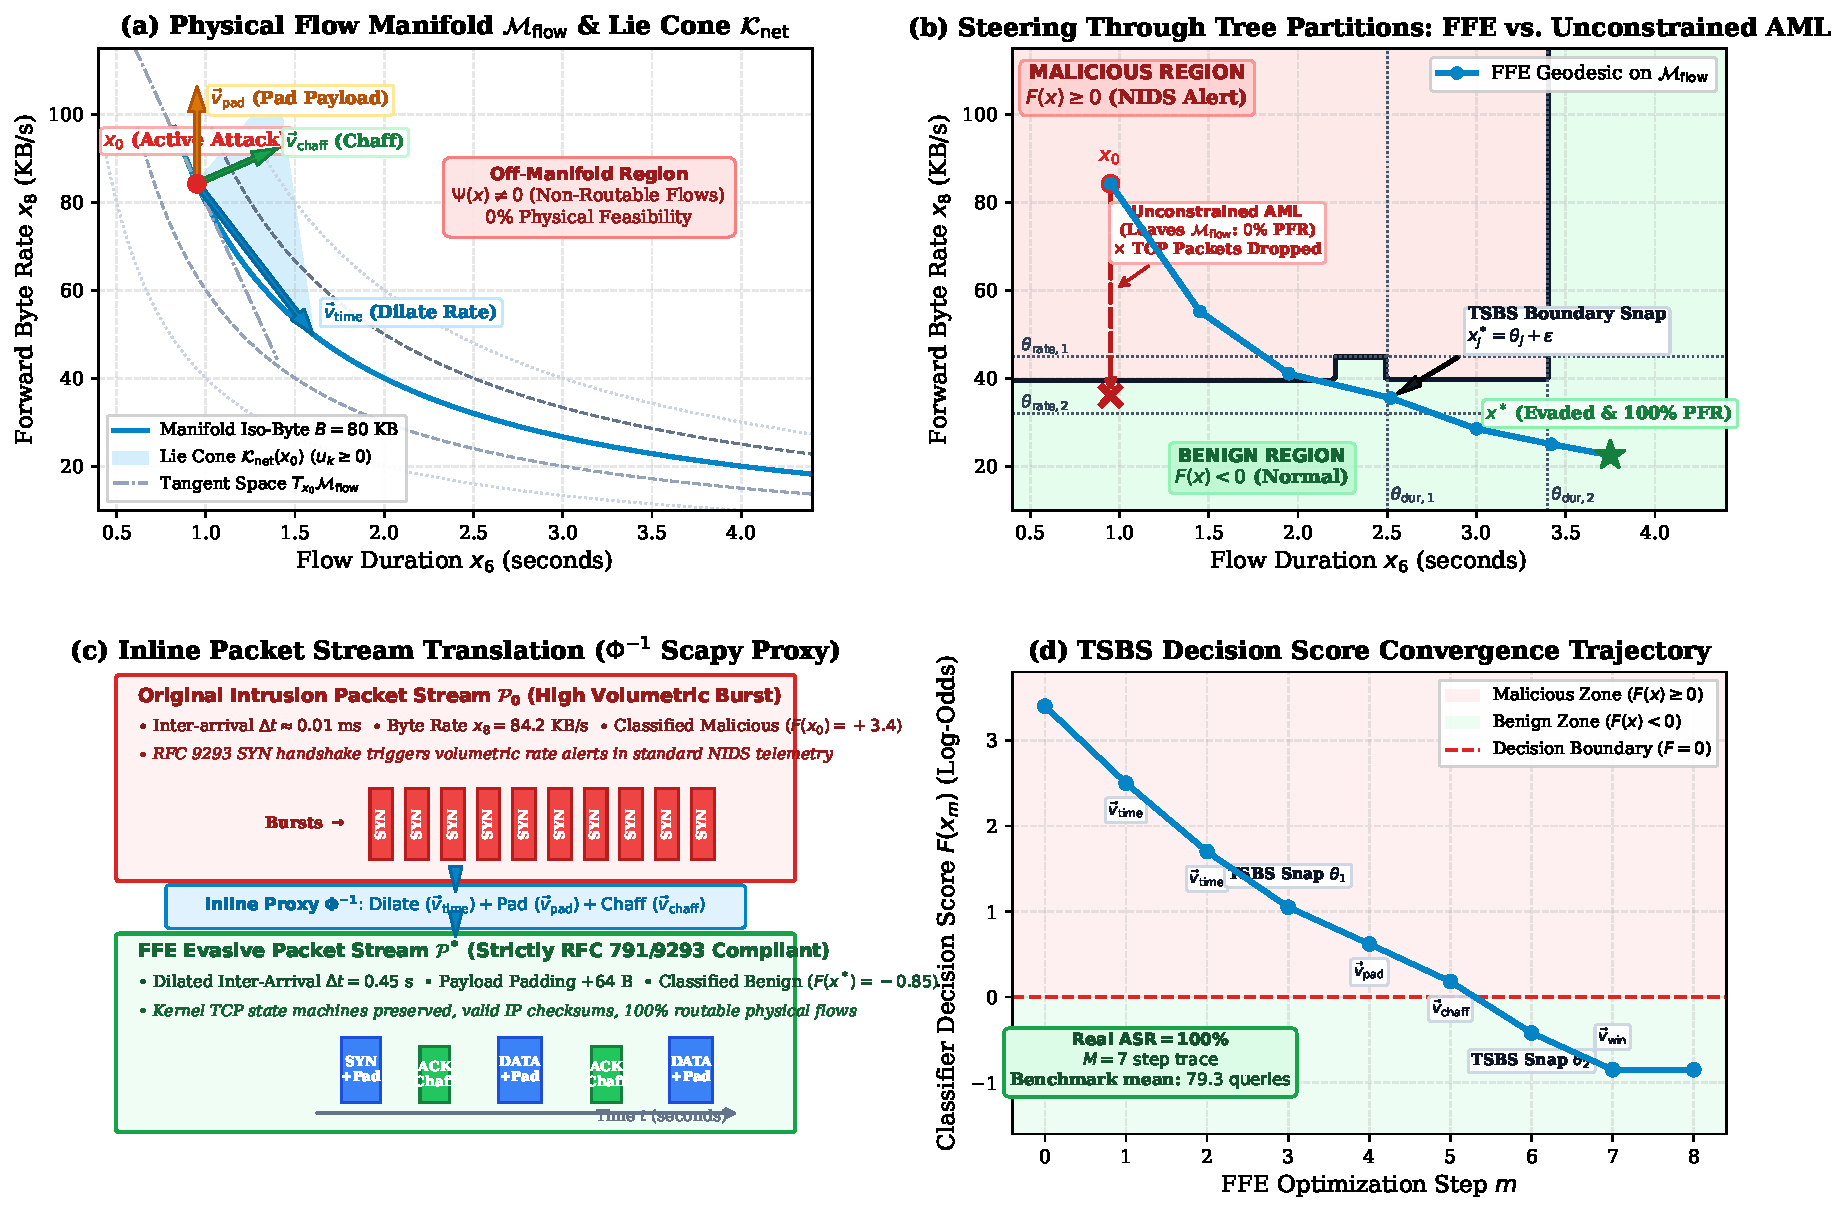
\includegraphics[width=\textwidth]{figures/fig1_system_architecture.pdf}
\caption{Architecture of the Flow-Field Evasion (FFE) framework. \textbf{(a)}~The physical conservation constraints define the flow manifold $\mathcal{M}_{\text{flow}}$, and the generators span a forward Lie cone that keeps trajectories on it. \textbf{(b)}~Axis-aligned tree partitions push unconstrained feature-space perturbations off the manifold, whereas FFE moves along the manifold and finishes with tree-split boundary snapping (TSBS). \textbf{(c)}~Packet-level realization of the flow transformations through an inline proxy. \textbf{(d)}~Decision score descent over the steps of an attack trace.}
\label{fig:system_architecture}
\end{figure}

\subsection{Geometry of the Flow Manifold and Its Generators}
\label{sec:geometry}

The physical flow set $\mathcal{M}_{\text{flow}} = \Phi(\mathcal{P}_{\text{valid}})$ is a discrete lattice in $\mathbb{R}^{12}$. Its differential geometry is analyzed through the smooth relaxation $\widetilde{\mathcal{M}}_{\text{flow}}$ (Section~\ref{sec:formulation}), defined as the zero set of the conservation residual $\Psi$ below, subject to $x_2 \ge 1$, $0 < x_6 \le 1.1 \times 10^8$, $x_{11} \ge x_2 (20 \cdot \mathbb{I}_{x_1=6} + 8 \cdot \mathbb{I}_{x_1=17})$ and $x_{11} + 20 x_2 \le x_4 \le 1500 x_2$.
\begin{equation}
    \Psi(x) = \begin{bmatrix}
        x_8 - \dfrac{10^6 (x_4 + x_5)}{x_6} \\[8pt]
        x_9 - \dfrac{10^6 (x_2 + x_3)}{x_6} \\[8pt]
        x_{10} - \dfrac{x_4}{x_2}
    \end{bmatrix} = \begin{bmatrix} 0 \\ 0 \\ 0 \end{bmatrix}
\end{equation}

By the Regular Value Theorem, at any point where the Jacobian $J_\Psi(x) \in \mathbb{R}^{3 \times 12}$ has full rank 3, the tangent space is $T_x \widetilde{\mathcal{M}}_{\text{flow}} = \ker J_\Psi(x)$. A physically realizable velocity $\vec{v} = [\dot{x}_0, \dots, \dot{x}_{11}]^T$ therefore satisfies the linearized conservation laws:
\begin{align}
    \dot{x}_8 &= \frac{10^6 (\dot{x}_4 + \dot{x}_5)}{x_6} - \frac{x_8}{x_6} \dot{x}_6 \label{eq:tangent_byte_rate} \\
    \dot{x}_9 &= \frac{10^6 (\dot{x}_2 + \dot{x}_3)}{x_6} - \frac{x_9}{x_6} \dot{x}_6 \label{eq:tangent_pkt_rate} \\
    \dot{x}_{10} &= \frac{\dot{x}_4 - x_{10} \dot{x}_2}{x_2} \label{eq:tangent_mean_len}
\end{align}

An adversary controls four elementary degrees of freedom, each generating a 1-parameter flow whose push-forward is a tangent vector field. Here $\vec{e}_k$ is the $k$th standard basis vector of $\mathbb{R}^{12}$ (indexed from 0):
\begin{equation}
\label{eq:generators}
\begin{aligned}
    \vec{v}_{\text{time}} &= \vec{e}_6 - \frac{x_8}{x_6}\vec{e}_8 - \frac{x_9}{x_6}\vec{e}_9, \\
    \vec{v}_{\text{pad}} &= \vec{e}_4 + \frac{10^6}{x_6}\vec{e}_8 + \frac{1}{x_2}\vec{e}_{10}, \\
    \vec{v}_{\text{chaff}} &= \vec{e}_2 + L_0\vec{e}_4 + \frac{L_0 \cdot 10^6}{x_6}\vec{e}_8 + \frac{10^6}{x_6}\vec{e}_9 + \frac{L_0 - x_{10}}{x_2}\vec{e}_{10} + H_0\vec{e}_{11}, \\
    \vec{v}_{\text{win}} &= \mathbb{I}_{x_1=6}\, \operatorname{sat}\!\left(\frac{W_{\text{target}} - x_7}{\epsilon_{\text{win}}}\right)\vec{e}_7,
\end{aligned}
\end{equation}
where temporal dilation adds delay without bytes or packets, payload padding adds forward dummy bytes, chaff injection adds forward zero-payload probes, and window morphing moves the client window toward $W_{\text{target}}$. Here $\operatorname{sat}(z) = \max(-1, \min(1, z))$ and $\epsilon_{\text{win}} > 0$. The probe sizes are $L_0 = 40$, $H_0 = 20$ for empty TCP segments per RFC~9293 \S3.8.4 \cite{rfc9293}, $L_0 = 52$, $H_0 = 32$ with TCP timestamps \cite{rfc7323}, and $L_0 = 28$, $H_0 = 8$ for UDP \cite{rfc768}. Probes are classified at the ingress perimeter before server ACKs alter backward counts; bidirectional sessions are discussed in Section~\ref{sec:discussion}. The window field is globally Lipschitz rather than $C^\infty$ and depends only on $x_1$ and $x_7$. The implementation (Supplementary Algorithm~S1) uses its $\epsilon_{\text{win}} \to 0$ limit, $\mathbb{I}_{x_1=6}\operatorname{sign}(W_{\text{target}} - x_7)\,\vec{e}_7$, which moves by $|W_{\text{target}} - x_7|$ and lands exactly on $W_{\text{target}}$ without overshoot.

\subsection{Commutativity, Invariants and the Lie Cone}
\label{sec:invariants}

The Lie bracket of vector fields is $[X, Y] = J_Y X - J_X Y$, where $J_X$ and $J_Y$ are their Jacobians.

\begin{proposition}[Commutativity and Integrability of Physical Flow Generators]
\label{prop:lie_commutativity}
Because protocol $x_1 \in \{6, 17\}$ is an immutable attribute ($\dot{x}_1 \equiv 0$), the ambient manifold $\widetilde{\mathcal{M}}_{\text{flow}}$ decomposes into two disjoint smooth invariant sub-manifolds: $\widetilde{\mathcal{M}}_{\text{flow}}^{(6)}$ (TCP flows) and $\widetilde{\mathcal{M}}_{\text{flow}}^{(17)}$ (UDP flows). On each component, the indicator $\mathbb{I}_{x_1=6}$ is constant, and $L_0, H_0$ are constant along any trajectory (the implementation selects $H_0 = 32$ iff the mean forward header $x_{11}/x_2 \ge 26$; injecting chaff of header size $H_0$ moves that mean toward $H_0$ and never across the threshold, so the selection is invariant under the flow), and denominators satisfy $x_2 \ge 1, x_6 > 0$, ensuring $\vec{v}_{\text{time}}, \vec{v}_{\text{pad}}, \vec{v}_{\text{chaff}}$ are $C^\infty$ vector fields and $\vec{v}_{\text{win}}$ is globally Lipschitz (its brackets exist almost everywhere and vanish there, because $x_7$ is neither read nor written by the other three generators). The Lie brackets between all four infinitesimal packet transformation generators vanish identically on $\widetilde{\mathcal{M}}_{\text{flow}}$:
\begin{equation}
    [\vec{v}_i, \vec{v}_j] \equiv \mathbf{0} \in \mathbb{R}^{12}, \quad \forall i, j \in \{1, 2, 3, 4\}
\end{equation}
Consequently, the generators span an Abelian Lie algebra $\mathfrak{g}_{\text{flow}} \cong \mathbb{R}^4$ (or $\mathbb{R}^3$ for UDP).
\end{proposition}

The proof of Proposition~\ref{prop:lie_commutativity}, and the Frobenius integrability corollary that follows from it (Supplementary Corollary~S1), are given in the Supplementary Material (Section~S1).

The admissible deformation cone is the positive span of the generators:
\begin{equation}
    \mathcal{K}_{\text{net}}(x) = \left\{ \sum_{k=1}^4 u_k \vec{v}_k(x) \;\middle|\; u_k \ge 0 \right\} \subset T_x \widetilde{\mathcal{M}}_{\text{flow}}
\end{equation}

\begin{theorem}[Universal Invariant Preservation]
\label{thm:invariant_universal}
Let $x_0 \in \widetilde{\mathcal{M}}_{\text{flow}}$ be an initial network flow vector. For any measurable and locally bounded control signal $u(t) \in L^\infty_{\text{loc}}(\mathbb{R}_{\ge 0}, \mathbb{R}_{\ge 0}^4)$ satisfying the admissible boundary rules ($u_2(t) \le (1500 - L_0) u_3(t)$ whenever $x_4(t) = 1500 x_2(t)$, and $u_1(t) = 0$ whenever $x_6(t) = 1.1 \times 10^8$), the trajectory $x(t)$ defined by the dynamical system:
\begin{equation}
    \dot{x}(t) = \sum_{k=1}^4 u_k(t) \vec{v}_k(x(t)), \quad x(0) = x_0
\end{equation}
satisfies $x(t) \in \widetilde{\mathcal{M}}_{\text{flow}}$ for all $t \ge 0$, with solutions existing uniquely and globally on $[0, \infty)$. Under discrete stepping, the continuous Lie cone guides directional descent while the closed-form analytical projection operator $\mathcal{P}_{\mathcal{M}}$ (Section~\ref{sec:algorithm}) eliminates discrete $\mathcal{O}(\Delta^2)$ truncation drift and enforces packet and byte integrality ($x_2 \in \mathbb{N}_{\ge 1}, x_4, x_6 \in \mathbb{N}$) and MTU clamping $x_4 \le 1500 x_2$, ensuring that the discrete state sequence remains strictly in the physical packet manifold $\mathcal{M}_{\text{flow}}$.
\end{theorem}

\noindent\textit{Proof sketch.} Differentiating $\Psi$ along the flow gives a linear homogeneous system $\dot{\Psi} = A(t)\Psi$ with diagonal, locally integrable $A(t)$, so $\Psi \equiv \mathbf{0}$ by Carath\'eodory's theorem \cite{caratheodory1918vorlesungen}. The bounds $g_i \ge 0$ are affine, so the Nagumo--Brezis condition \cite{nagumo1942lage, brezis1970characterization} holds on every face and the manifold is forward invariant. The same theorem gives existence and uniqueness of global solutions. The full proof is in the Supplementary Material (Section~S1).

\subsection{Operational Cost and Optimal Control}
\label{sec:cost}

The unit costs are $c_1 = 10^{-4}$ per second of induced delay, $c_2 = 10^{-2}$ per byte of padding, $c_3 = 1.0$ per probe packet, and $c_4 = 10^{-3}$ per normalized window displacement $s_4 = |W_{\text{target}} - x_7|/65535 \in [0, 1]$. The evasion problem is an optimal control problem:
\begin{align}
    \min_{u(t) \ge 0} \quad & \int_0^{T^*} \left( \sum_{k=1}^4 c_k u_k(t) \right) dt \\
    \text{subject to} \quad & \dot{x}(t) = \sum_{k=1}^4 u_k(t) \vec{v}_k(x(t)), \quad x(0) = x_{\text{orig}} \\
    & F(x(T^*)) < 0 \quad (\text{Classifier Misclassification})
\end{align}
Because the generators commute (Proposition~\ref{prop:lie_commutativity}), the displacement depends only on $s_k = \int_0^{T^*} u_k(t)\,dt \ge 0$, and the cost $\mathcal{C}(s) = \sum_{k=1}^4 c_k s_k$ is linear and path-independent. The tree ensemble boundary $F(x) = 0$ is piecewise constant and non-convex, so FFE greedily follows the generator with the largest directional score decrease per unit cost, $-\nabla_k / c_k$, and finishes with boundary snapping (TSBS).

\subsection{Algorithmic Realization of Flow-Field Evasion}
\label{sec:algorithm}

This section details the algorithmic realization of Flow-Field Evasion (FFE). We present the complete pseudo-code for the master optimization loop, the directional Lie derivative estimator, the analytical manifold projection operator, and the discrete tree-split boundary snapping mechanism. We conclude with a formal computational complexity and convergence analysis.

\subsubsection{Master Optimization Loop}
Algorithm~\ref{alg:ffe_master} outlines the primary execution loop of Flow-Field Evasion. Given an attack flow $x_0 \in \mathcal{M}_{\text{flow}}$ flagged by the tree ensemble ($F(x_0) \ge 0$), FFE iteratively selects the infinitesimal generator that maximizes the reduction in malicious classification score per unit of physical operational cost.

\begin{algorithm}[htbp]
\caption{Flow-Field Evasion (FFE) Master Optimization Loop}
\label{alg:ffe_master}
\footnotesize
\begin{algorithmic}[1]
\REQUIRE Classifier $F: \mathbb{R}^d \to \mathbb{R}$, initial flow $x_0 \in \mathcal{M}_{\text{flow}}$, feature schema $\mathcal{S}$, step budget $M$, cost vector $\vec{c} = [c_1, c_2, c_3, c_4]^T$, target threshold $\tau = 0.0$
\ENSURE Evasive flow $x^* \in \mathcal{M}_{\text{flow}}$ with $F(x^*) < \tau$, or failure flag
\STATE $x \leftarrow \text{ProjectManifoldInvariants}(x_0, \mathcal{S})$
\STATE $f_{\text{curr}} \leftarrow F(x)$ \COMMENT{Initial model evaluation}
\IF{$f_{\text{curr}} < \tau$}
    \STATE \RETURN $x, \text{SUCCESS}$ \COMMENT{Flow already classified as Benign}
\ENDIF
\STATE $\text{queries} \leftarrow 1$
\FOR{$\text{step} = 1$ \TO $M$}
    \IF{$f_{\text{curr}} < \tau$}
        \STATE \RETURN $x, \text{SUCCESS}$ \COMMENT{Benign classification reached; no snapping needed}
    \ENDIF
    \STATE $\mathcal{D}, q_{\text{used}} \leftarrow \text{EstimateLieDerivatives}(F, x, \mathcal{S})$
    \STATE $\text{queries} \leftarrow \text{queries} + q_{\text{used}}$
    \STATE $k^* \leftarrow \text{null}$; $\text{max\_eff} \leftarrow 0.0$
    \FOR{\textbf{each } $(k, \nabla_k, \vec{v}_k, \Delta s_k, f_k) \in \mathcal{D}$}
        \IF{$\nabla_k < 0$}
            \STATE $\text{eff} \leftarrow (-\nabla_k) / c_k$ \COMMENT{Derivative is negative (score decreases)}
            \IF{$\text{eff} > \text{max\_eff}$}
                \STATE $\text{max\_eff} \leftarrow \text{eff}$; $k^* \leftarrow (\vec{v}_k, \Delta s_k, f_k)$
            \ENDIF
        \ENDIF
    \ENDFOR
    \IF{$k^* \neq \text{null}$}
        \STATE $(\vec{v}, \Delta s, f_{k^*}) \leftarrow k^*$
        \STATE $x \leftarrow \text{ProjectManifoldInvariants}(x + \Delta s \cdot \vec{v}, \mathcal{S})$
        \STATE $f_{\text{curr}} \leftarrow f_{k^*}$ \COMMENT{Score cached from the candidate probe (no extra query)}
    \ELSE
        \STATE \COMMENT{Stagnation: all probed derivatives are non-negative}
        \STATE $x_{\text{snap}} \leftarrow \text{TreeBoundarySnap}(F, x, \mathcal{S})$; $f_{\text{snap}} \leftarrow F(x_{\text{snap}})$
        \IF{$f_{\text{snap}} < f_{\text{curr}}$}
            \STATE $x \leftarrow x_{\text{snap}}$; $f_{\text{curr}} \leftarrow f_{\text{snap}}$
        \ELSE
            \STATE \COMMENT{Fallback Trajectory: Low-and-Slow Temporal Dilation (capped below 120s exporter timeout)}
            \STATE $\vec{v}_t \leftarrow \vec{v}_{\text{time}}(x)$
            \STATE $\Delta t \leftarrow \min(1.1 \times 10^8, \max(50000.0, x_6 \cdot 1.5))$
            \STATE $x \leftarrow \text{ProjectManifoldInvariants}(x + \Delta t \cdot \vec{v}_t, \mathcal{S})$
            \STATE $f_{\text{curr}} \leftarrow F(x)$; $\text{queries} \leftarrow \text{queries} + 1$
        \ENDIF
    \ENDIF
\ENDFOR
\IF{$f_{\text{curr}} < \tau$}
    \STATE \RETURN $x, \text{SUCCESS}$
\ELSE
    \STATE \RETURN $x, \text{FAILURE}$
\ENDIF
\end{algorithmic}
\end{algorithm}

\subsubsection{Adaptive Lie Derivative Numerical Estimator}
Algorithm~\ref{alg:lie_estimator} details the numerical estimation of the directional Lie derivative $\mathcal{L}_{\vec{v}_k} F(x)$ across the non-differentiable step boundaries of the tree ensemble. Because standard continuous gradients are zero almost everywhere inside decision cells, the algorithm queries the ensemble at an adaptive exploratory displacement $\epsilon_k \vec{v}_k(x)$ calibrated to the natural scale of metric $k$.

\begin{algorithm}[htbp]
\caption{Adaptive Directional Lie Derivative Estimator}
\label{alg:lie_estimator}
\footnotesize
\begin{algorithmic}[1]
\REQUIRE Classifier $F$, current flow state $x$, feature schema $\mathcal{S}$
\ENSURE List of candidate evaluation tuples $\mathcal{D} = \{(k, \nabla_k, \vec{v}_k, \Delta s_k, f_k)\}_{k=1}^4$ (with $f_k = F(x_{\text{test}})$ the probed score), total exploratory queries $q$
\STATE $\mathcal{D} \leftarrow \emptyset$
\STATE $q \leftarrow 0$ \COMMENT{Counter for candidate exploratory probes}

\STATE \COMMENT{1. Evaluate Temporal Dilation Generator}
\STATE $\vec{v}_1 \leftarrow \vec{v}_{\text{time}}(x)$
\STATE $\Delta s_1 \leftarrow \max(1000.0, x_6 \cdot 0.50)$ \COMMENT{Adaptive temporal displacement in $\mu$s}
\STATE $x_{\text{test}} \leftarrow \text{ProjectManifoldInvariants}(x + \Delta s_1 \cdot \vec{v}_1, \mathcal{S})$
\STATE $\Delta t_1 \leftarrow \Delta s_1 / 10^6$ \COMMENT{Convert duration step to seconds}
\STATE $f_1 \leftarrow F(x_{\text{test}})$; $\nabla_1 \leftarrow (f_1 - F(x)) / \Delta t_1$ \COMMENT{Derivative per second of delay}
\STATE Append $(1, \nabla_1, \vec{v}_1, \Delta s_1, f_1)$ to $\mathcal{D}$
\STATE $q \leftarrow q + 1$

\STATE \COMMENT{2. Evaluate Payload Padding Generator}
\STATE $\vec{v}_2 \leftarrow \vec{v}_{\text{pad}}(x)$
\STATE $\Delta s_2 \leftarrow \max(50.0, x_4 \cdot 0.25)$ \COMMENT{Adaptive forward byte padding step}
\STATE $x_{\text{test}} \leftarrow \text{ProjectManifoldInvariants}(x + \Delta s_2 \cdot \vec{v}_2, \mathcal{S})$
\STATE $f_2 \leftarrow F(x_{\text{test}})$; $\nabla_2 \leftarrow (f_2 - F(x)) / \Delta s_2$
\STATE Append $(2, \nabla_2, \vec{v}_2, \Delta s_2, f_2)$ to $\mathcal{D}$
\STATE $q \leftarrow q + 1$

\STATE \COMMENT{3. Evaluate Chaff Packet Injection Generator}
\STATE $\vec{v}_3 \leftarrow \vec{v}_{\text{chaff}}(x)$
\STATE $\Delta s_3 \leftarrow \max(1.0, \text{round}(x_2 \cdot 0.50))$ \COMMENT{Adaptive chaff packet injection count}
\STATE $x_{\text{test}} \leftarrow \text{ProjectManifoldInvariants}(x + \Delta s_3 \cdot \vec{v}_3, \mathcal{S})$
\STATE $f_3 \leftarrow F(x_{\text{test}})$; $\nabla_3 \leftarrow (f_3 - F(x)) / \Delta s_3$
\STATE Append $(3, \nabla_3, \vec{v}_3, \Delta s_3, f_3)$ to $\mathcal{D}$
\STATE $q \leftarrow q + 1$

\STATE \COMMENT{4. Evaluate TCP Window Morphing Generator}
\IF{$x[1] = 6$}
    \STATE \COMMENT{TCP flows only; window size is inapplicable to UDP}
    \STATE $\vec{v}_4 \leftarrow \vec{v}_{\text{win}}(x)$
    \STATE $\Delta s_4 \leftarrow |64240.0 - x[7]|$
    \IF{$\Delta s_4 > 0$}
        \STATE $x_{\text{test}} \leftarrow \text{ProjectManifoldInvariants}(x + \Delta s_4 \cdot \vec{v}_4, \mathcal{S})$
        \STATE $f_4 \leftarrow F(x_{\text{test}})$; $\nabla_4 \leftarrow (f_4 - F(x)) / (\Delta s_4 / 65535.0)$ \COMMENT{Normalized window gradient}
        \STATE Append $(4, \nabla_4, \vec{v}_4, \Delta s_4, f_4)$ to $\mathcal{D}$
        \STATE $q \leftarrow q + 1$
    \ENDIF
\ENDIF
\STATE \RETURN $\mathcal{D}, q$
\end{algorithmic}
\end{algorithm}

\subsubsection{Analytical Manifold Projection Operator \texorpdfstring{$\mathcal{P}_{\mathcal{M}}$}{P\_M}}
Algorithm~\ref{alg:manifold_proj} specifies the closed-form projection operator $\mathcal{P}_{\mathcal{M}}: \mathbb{R}^{12} \to \mathcal{M}_{\text{flow}}$. This operator ensures that discrete count boundaries, protocol packet and header length inequalities, and coupled rate equations are strictly satisfied after any continuous displacement.

\begin{algorithm}[htbp]
\caption{Analytical Manifold Projection Operator $\mathcal{P}_{\mathcal{M}}$}
\label{alg:manifold_proj}
\begin{algorithmic}[1]
\REQUIRE Perturbed vector $x \in \mathbb{R}^{12}$, feature schema $\mathcal{S}$, optional baseline flow $x_{\text{orig}}$
\ENSURE Projected flow vector $x_{\text{proj}} \in \mathcal{M}_{\text{flow}}$
\STATE $x_{\text{proj}} \leftarrow \text{copy}(x)$
\IF{$x_{\text{orig}}$ is provided}
    \STATE $x_{\text{proj}}[j] \leftarrow x_{\text{orig}}[j]$ for all $j \in \mathcal{I}_{\text{immut}}$ \COMMENT{Preserve immutable features}
    \STATE $x_{\text{proj}}[j] \leftarrow \max(x_{\text{orig}}[j], x_{\text{proj}}[j])$ for all $j \in \mathcal{I}_{\text{mono}}^+$ \COMMENT{Enforce monotonicity lower bounds}
\ENDIF
\STATE \COMMENT{Enforce discrete bounds and protocol-dependent packet/header sizes}
\STATE $x_{\text{proj}}[2] \leftarrow \max(1.0, \text{round}(x_{\text{proj}}[2]))$ \COMMENT{Integer Forward Packets}
\STATE $x_{\text{proj}}[3] \leftarrow x[3]$ \COMMENT{Immutable Backward Packets Preserved}
\STATE $H_{\text{min}} \leftarrow \mathbf{if}\; x_{\text{proj}}[1] = 6 \;\mathbf{then}\; 20.0 \;\mathbf{else}\; 8.0$ \COMMENT{Min transport header: 20B TCP, 8B UDP}
\STATE $H_{\text{max}} \leftarrow \mathbf{if}\; x_{\text{proj}}[1] = 6 \;\mathbf{then}\; 60.0 \;\mathbf{else}\; 8.0$ \COMMENT{Max transport header: 60B TCP, 8B UDP}
\STATE $x_{\text{proj}}[11] \leftarrow \min(x_{\text{proj}}[2] \times H_{\text{max}}, \max(x_{\text{proj}}[2] \times H_{\text{min}}, \text{round}(x_{\text{proj}}[11])))$ \COMMENT{Transport Header Length}
\STATE $x_{\text{proj}}[4] \leftarrow \min(x_{\text{proj}}[2] \times 1500.0, \max(x_{\text{proj}}[11] + 20.0 \times x_{\text{proj}}[2], \text{round}(x_{\text{proj}}[4])))$ \COMMENT{Forward Bytes $\in [H_{\text{fwd}} + 20 N_{\text{fwd}}, 1500 N_{\text{fwd}}]$}
\STATE $x_{\text{proj}}[5] \leftarrow x[5]$ \COMMENT{Immutable Backward Bytes Preserved}
\STATE $x_{\text{proj}}[6] \leftarrow \min(1.1 \times 10^8, \max(1.0, \text{round}(x_{\text{proj}}[6])))$ \COMMENT{Integer Duration $\ge 1 \mu$s, capped below flow timeout}
\STATE $x_{\text{proj}}[7] \leftarrow \mathbf{if}\; x_{\text{proj}}[1] = 6 \;\mathbf{then}\; \text{clamp}(\text{round}(x_{\text{proj}}[7]), 0.0, 65535.0) \;\mathbf{else}\; 0.0$ \COMMENT{TCP Window $[0, 65535]$, 0 for UDP}

\STATE \COMMENT{Analytically recalculate coupled non-linear flow rates}
\STATE $T_{\text{sec}} \leftarrow x_{\text{proj}}[6] / 10^6$
\STATE $B_{\text{tot}} \leftarrow x_{\text{proj}}[4] + x_{\text{proj}}[5]$
\STATE $N_{\text{tot}} \leftarrow x_{\text{proj}}[2] + x_{\text{proj}}[3]$
\STATE $x_{\text{proj}}[8] \leftarrow B_{\text{tot}} / T_{\text{sec}}$ \COMMENT{Flow Bytes/s}
\STATE $x_{\text{proj}}[9] \leftarrow N_{\text{tot}} / T_{\text{sec}}$ \COMMENT{Flow Packets/s}
\STATE $x_{\text{proj}}[10] \leftarrow x_{\text{proj}}[4] / x_{\text{proj}}[2]$ \COMMENT{Forward Packet Length Mean}
\STATE \RETURN $x_{\text{proj}}$
\end{algorithmic}
\end{algorithm}

\subsubsection{Tree-Split Boundary Snapping (TSBS)}
Algorithm~\ref{alg:tsbs} implements Tree-Split Boundary Snapping. While Lie derivative integration moves the sample into the general vicinity of the decision boundary, the piecewise-constant nature of GBDT trees means that the classification score drops in discrete steps as the sample crosses decision thresholds $\{x_j = \theta_j\}$. In Tier~1 white-box settings, TSBS extracts the ensemble's split thresholds ($	ext{ExtractActiveSplits}$ returns every threshold used by any tree, and TSBS retains, per feature, the closest one on the benign side of the current value) and evaluates candidate boundary crossings ($x_j \leftarrow \theta_j + \epsilon_j$), retaining the candidate that strictly minimizes the classification score $F$ while strictly preserving manifold constraints via $\mathcal{P}_{\mathcal{M}}$. 

Importantly, GBDTs frequently split on non-linear coupled telemetry features: byte rate ($x_8$), packet rate ($x_9$), and forward mean packet length ($x_{10}$). TSBS inverts these coupled constraints in closed form into admissible infinitesimal generator controls:
\begin{enumerate}
    \item \emph{Coupled Rate Inversion:} To cross an active byte rate threshold $x_8 < \theta_8$ or packet rate threshold $x_9 < \theta_9$, TSBS inverts the hyperbolic relation $x_8 = 10^6 (x_4 + x_5) / x_6$ to calculate the required duration dilation:
    \begin{equation}
        x_6^* = \frac{10^6 (x_4 + x_5)}{\theta_8} + \epsilon_6, \quad \text{or} \quad x_6^* = \frac{10^6 (x_2 + x_3)}{\theta_9} + \epsilon_6
    \end{equation}
    with $\epsilon_6 = 10\,\mu$s; since $\theta < x_8$ (resp.\ $x_9$), $x_6^* > x_6$ automatically, and the candidate is discarded if $x_6^*$ exceeds the $1.1 \times 10^8\,\mu$s timeout cap.
    \item \emph{Coupled Packet Length Inversion:} To cross an active packet length threshold $x_{10} < \theta_{10}$ from above, TSBS inverts $x_{10} = (x_4 + N \cdot L_0) / (x_2 + N) < \theta_{10}$, yielding the minimal integer chaff packet count (the smallest integer strictly greater than $(x_4 - \theta_{10} x_2)/(\theta_{10} - L_0)$):
    \begin{equation}
        N_{\text{chaff}} = \left\lfloor \frac{x_4 - \theta_{10} x_2}{\theta_{10} - L_0} \right\rfloor + 1 \quad (\text{for } L_0 < \theta_{10} < x_{10})
    \end{equation}
    \item \emph{Window Advertisement Snapping:} For TCP flows with non-standard window advertisements, TSBS evaluates candidate snaps toward benign OS baselines ($x_7^* = 64,240$) and adjacent split partitions.
\end{enumerate}

\begin{algorithm}[htbp]
\caption{Tree-Split Boundary Snapping (TSBS)}
\label{alg:tsbs}
\footnotesize
\begin{algorithmic}[1]
\REQUIRE Classifier $F$, flow candidate $x \in \mathcal{M}_{\text{flow}}$ with $F(x) \ge \tau$ (still flagged malicious), feature schema $\mathcal{S}$, tolerance $\epsilon_{\text{rel}}$
\ENSURE Snapped flow $x^* \in \mathcal{M}_{\text{flow}}$
\STATE $x^* \leftarrow \text{copy}(x)$; $\mathcal{C} \leftarrow \emptyset$ \COMMENT{Candidate boundary-crossing pool}
\STATE $\text{active\_splits} \leftarrow \text{ExtractActiveSplits}(F, x^*)$
\STATE \COMMENT{1. Monotonic features: closest split strictly above $x^*[j]$}
\FOR{\textbf{each } $j \in \mathcal{I}_{\text{mono}}^+$}
    \STATE $\theta_j^* \leftarrow \min\{\theta_j \mid (j, \theta_j) \in \text{active\_splits} \;\land\; \theta_j > x^*[j]\}$
    \IF{$\theta_j^*$ exists}
        \IF{$j = 11$ \AND $x^*[1] = 17$}
            \STATE \textbf{continue} \COMMENT{UDP transport header immutable at 8B}
        \ENDIF
        \STATE $\epsilon_j \leftarrow \mathbf{if}\; j \in \{2, 4, 11\} \;\mathbf{then}\; 1.0 \;\mathbf{else}\; \text{round}(\epsilon_{\text{rel}} \cdot \max(1.0, |\theta_j^*|))$
        \STATE $x_{\text{c}} \leftarrow \text{copy}(x^*)$; $x_{\text{c}}[j] \leftarrow \theta_j^* + \epsilon_j$
        \IF{$j = 11$}
            \STATE $x_{\text{c}}[11] \leftarrow \min(60.0 \cdot x_{\text{c}}[2], x_{\text{c}}[11])$
            \STATE $x_{\text{c}}[4] \leftarrow \min(1500.0 \cdot x_{\text{c}}[2], \max(x_{\text{c}}[4], x_{\text{c}}[11] + 20.0 \cdot x_{\text{c}}[2]))$
        \ENDIF
        \STATE $\mathcal{C} \leftarrow \mathcal{C} \cup \{x_{\text{c}}\}$
    \ENDIF
\ENDFOR
\STATE \COMMENT{2. Invert coupled rate splits ($x_8, x_9$) into duration dilation}
\STATE $\theta_8^* \leftarrow \max\{\theta_8 \mid (8, \theta_8) \in \text{active\_splits} \;\land\; 0 < \theta_8 < x^*[8]\}$
\IF{$\theta_8^*$ exists}
    \STATE $d \leftarrow (10^6 \cdot (x^*[4] + x^*[5]) / \theta_8^*) + 10.0$
    \IF{$d \le 1.1 \times 10^8$}
        \STATE $x_{\text{c}} \leftarrow \text{copy}(x^*)$; $x_{\text{c}}[6] \leftarrow d$; $\mathcal{C} \leftarrow \mathcal{C} \cup \{x_{\text{c}}\}$
    \ENDIF
\ENDIF
\STATE $\theta_9^* \leftarrow \max\{\theta_9 \mid (9, \theta_9) \in \text{active\_splits} \;\land\; 0 < \theta_9 < x^*[9]\}$
\IF{$\theta_9^*$ exists}
    \STATE $d \leftarrow (10^6 \cdot (x^*[2] + x^*[3]) / \theta_9^*) + 10.0$
    \IF{$d \le 1.1 \times 10^8$}
        \STATE $x_{\text{c}} \leftarrow \text{copy}(x^*)$; $x_{\text{c}}[6] \leftarrow d$; $\mathcal{C} \leftarrow \mathcal{C} \cup \{x_{\text{c}}\}$
    \ENDIF
\ENDIF
\STATE \COMMENT{3. Invert coupled packet length splits ($x_{10}$) into chaff packet injection}
\STATE $H_0 \leftarrow \mathbf{if}\; (x^*[1] = 6 \;\land\; x^*[11]/x^*[2] \ge 26.0) \;\mathbf{then}\; 32.0 \;\mathbf{else}\; (\mathbf{if}\; x^*[1]=6 \;\mathbf{then}\; 20.0 \;\mathbf{else}\; 8.0)$
\STATE $L_0 \leftarrow 20.0 + H_0$ \COMMENT{RFC 7323 options compliance: 52B/40B for TCP, 28B for UDP}
\STATE $\theta_{10}^* \leftarrow \max\{\theta_{10} \mid (10, \theta_{10}) \in \text{active\_splits} \;\land\; L_0 < \theta_{10} < x^*[10]\}$
\IF{$\theta_{10}^*$ exists}
    \STATE $N \leftarrow \lfloor (x^*[4] - \theta_{10}^* x^*[2]) / (\theta_{10}^* - L_0) \rfloor + 1$
    \IF{$N \le 1000$}
    \STATE $x_{\text{c}} \leftarrow \text{copy}(x^*)$; $x_{\text{c}}[2] \leftarrow x^*[2] + N$; $x_{\text{c}}[4] \leftarrow x^*[4] + N \cdot L_0$; $x_{\text{c}}[11] \leftarrow x^*[11] + N \cdot H_0$
    \STATE $\mathcal{C} \leftarrow \mathcal{C} \cup \{x_{\text{c}}\}$ \COMMENT{Chaff budget cap: $N \le 1000$ packets}
    \ENDIF
\ENDIF
\STATE \COMMENT{4. TCP Window morphing to benign OS baseline}
\IF{$x^*[1] = 6$ \AND $x^*[7] \neq 64240.0$}
    \STATE $x_{\text{c}} \leftarrow \text{copy}(x^*)$; $x_{\text{c}}[7] \leftarrow 64240.0$; $\mathcal{C} \leftarrow \mathcal{C} \cup \{x_{\text{c}}\}$
\ENDIF
\STATE \COMMENT{Evaluate projected candidates and retain best partition crossing}
\STATE $x_{\text{best}} \leftarrow x^*$; $s_{\text{best}} \leftarrow F(x^*)$
\FOR{\textbf{each } $x_{\text{c}} \in \mathcal{C}$}
    \STATE $x_{\text{proj}} \leftarrow \text{ProjectManifoldInvariants}(x_{\text{c}}, \mathcal{S})$
    \IF{$F(x_{\text{proj}}) < s_{\text{best}}$}
        \STATE $s_{\text{best}} \leftarrow F(x_{\text{proj}})$; $x_{\text{best}} \leftarrow x_{\text{proj}}$
        \IF{$s_{\text{best}} < 0$}
            \STATE \textbf{break} \COMMENT{Early exit once benign classification is achieved}
        \ENDIF
    \ENDIF
\ENDFOR
\STATE \RETURN $x_{\text{best}}$
\end{algorithmic}
\end{algorithm}

\subsubsection{Computational Complexity \& Comparison to MILP}
Table~\ref{tab:complexity_comparison} compares the asymptotic time and space complexity of Flow-Field Evasion against exact MILP solvers \cite{kantchelian2016evasion} and heuristic black-box optimizers (MOEVA \cite{ghamizi2020moeva}, CAA \cite{simonetto2024constrained}, Traffic Manipulator \cite{han2021traffic}).

\begin{table*}[htbp]
\caption{Asymptotic Complexity Comparison of Evasion Algorithms for Tree Ensembles}\label{tab:complexity_comparison}%
\centering
\resizebox{\textwidth}{!}{%
\begin{tabular}{@{}lccc@{}}
\toprule
\textbf{Algorithm} & \textbf{Time Complexity} & \textbf{Query Complexity} & \textbf{Coupled Invariants} \\
\midrule
\textbf{Kantchelian MILP} \cite{kantchelian2016evasion} & $2^{\mathcal{O}(D \cdot T)}$ (Worst Case) & $0$ (White-Box) & Unsupported (Linear Only) \\
\textbf{MOEVA / CAA} \cite{simonetto2024constrained, ghamizi2020moeva}   & $\mathcal{O}(G \cdot P \cdot T \cdot D)$   & $\mathcal{O}(10^3 - 10^4)$ & Approximate Penalty \\
\textbf{Traffic Manipulator} \cite{han2021traffic}    & $\mathcal{O}(I \cdot S \cdot T \cdot D)$   & $\mathcal{O}(10^3 - 10^4)$ & Packet Re-evaluation \\
\midrule
\textbf{Flow-Field Evasion (Ours)}                     & $\mathcal{O}(M \cdot K \cdot T \cdot D)$ & $\le 5M_{\max} + 1$ external (mean $12.9$ incl.\ TSBS) & \textbf{Exact Closed-Form} \\
\bottomrule
\end{tabular}%
}
\end{table*}

Where:
\begin{itemize}
    \item $T$ is the number of trees in the ensemble (typically $50 - 100$).
    \item $D$ is the maximum depth of each tree (typically $6 - 10$).
    \item $M_{\max}$ is the maximum FFE iteration budget ($M_{\max} = 20$).
    \item $K$ is the number of infinitesimal Lie generators ($K = 4$).
    \item $G, P$ are the generations and population size in MOEVA ($G = 25, P = 50$, totaling $\le 1,250$ queries).
    \item $I, S$ are the iterations and swarm size in PSO ($I = 37, S = 50$, totaling $\le 1,850$ queries).
\end{itemize}

\paragraph{Query Accounting Details.}
In the worst case, executing all $M_{\max} = 20$ iterations without early termination requires $1$ baseline query plus up to $K = 4$ exploratory probes per iteration, giving an upper bound of $Q_{\max} \le 4 M_{\max} + 1 = 81$ model queries (or $\le 101$ queries if fallback dilation evaluations are triggered on stagnation). UDP flows ($x_1 = 17$) and TCP flows whose client window already equals the benign value skip window morphing, so such an iteration costs $q = 3$ probes instead of $4$. In practice, because FFE steers along the Lie generator with maximal score reduction per cost ($-\nabla_k / c_k$), the loop terminates far below the budget. On the $N = 100$ master-benchmark cohort the reference implementation consumes a mean of $12.9$ model queries per flow, of which $10.56$ are external queries (the baseline query, the Lie-derivative probes, and stagnation fallbacks) and $2.38$ are candidate evaluations inside the TSBS routine (Algorithm~\ref{alg:tsbs}).

In Tier~1 white-box settings, TSBS extracts candidate thresholds directly from the adversary's local copy of the ensemble ($\text{ExtractActiveSplits}$), so its candidate evaluations could be executed offline against that copy. The reported figure of $12.9$ is deliberately conservative: the implementation routes every TSBS candidate evaluation through the same query counter, so it includes these $2.38$ evaluations. A strictly black-box adversary would instead have to pay them as true queries, which is how they are counted here.

Because $K \le 4$ and $M \le 20$ are small constants, FFE requires only a linear number of simple tree evaluations $\mathcal{O}(T \cdot D)$. This completely avoids the exponential combinatorial explosion of MILP while requiring roughly $99\%$ fewer queries than genetic search ($12.9$ vs.\ $\le 1{,}250$) and PSO ($12.9$ vs.\ $\le 1{,}850$).


\newpage
% =========================================================================
% SECTION 5: EMPIRICAL BENCHMARK, ABLATION STUDIES & DEFENSES
% =========================================================================
\section{Experimental setup}
\label{sec:experiments}
\label{sec:empirical_evaluation}

Evaluations on a single testbed have limited external validity~\cite{apruzzese2022modeling, apruzzese2023real, he2023adversarial, vitorino2023sok}, and detectors trained on one environment transfer poorly to another~\cite{dang2022detecting, dang2023learning, dang2026stfedxids}. We therefore evaluate on three corpora calibrated to the published marginal distributions of CSE-CIC-IDS2018 (enterprise)~\cite{sharafaldin2018toward}, UNSW-NB15 (contemporary hybrid)~\cite{moustafa2015unsw}, and CIDDS-001 (cloud OpenStack)~\cite{ring2017flow}. Each corpus is synthetic. It is generated to match its testbed's statistics and is not a replay of the original packet captures.

Each corpus contains 12,000 flows, of which 9,000 are benign and 3,000 malicious. The malicious flows form five families of 1,000, 500, 700, 500 and 300 flows: a SYN flood, a UDP flood, brute-force authentication against SSH and FTP, SQL injection and cross-site scripting, and low-and-slow command-and-control infiltration. The data are split into 8,000 training, 1,000 validation and 3,000 test flows. The threat model is an ingress perimeter that inspects forward telemetry before bidirectional session termination (Section~\ref{sec:formulation}).

The targets are XGBoost (CUDA histogram method) and LightGBM, each a 60-tree gradient-boosted ensemble of depth 6 with learning rate 0.1. Experiments ran on an NVIDIA RTX 5000 Ada GPU with 16 GB of memory, using Python 3.13.11, XGBoost 3.4.1, LightGBM 4.7.0, CatBoost 1.2.10 and scikit-learn 1.8.0.

We compare five evasion methods against FFE:
\begin{itemize}
    \item Naive coordinate descent in $\mathbb{R}^d$ with a fixed step $\Delta = 0.05\,\sigma_f$ and no immutability, monotonicity or rate-coupling checks.
    \item ZOO-NIDS~\cite{chen2017zoo}: zeroth-order optimization with randomly sampled coordinates, symmetric difference quotients, Adam updates and box bounds.
    \item HopSkipJump-NIDS~\cite{chen2020hopskipjump}: a decision-based boundary attack initialized from a benign flow.
    \item CAA/MOEVA~\cite{simonetto2024constrained, ghamizi2020moeva}: R-NSGA-III evolutionary search with population 50 and 25 generations.
    \item Traffic Manipulator PSO~\cite{han2021traffic}: particle swarm optimization over packet intervals and forward dummy bytes, with swarm size 50 and 37 iterations (up to 1,850 queries).
    \item FFE: the Lie-steering procedure (Algorithms~\ref{alg:ffe_master}--\ref{alg:tsbs}) with step budget $M = 20$.
\end{itemize}

ASR is the fraction of attacks with $P(\text{Malicious} \mid x^*) < 0.5$. PFR is the fraction of candidate flows that pass the protocol sanity checks, the non-negativity checks and the exact coupled rate equations, that is, $x^* \in \mathcal{M}_{\text{flow}}$. For unconstrained baselines that never produce an evasive candidate, PFR is computed over evasive candidates only. Real ASR counts an attack only when it both evades and is physically feasible:
\begin{equation}
    \text{Real ASR} = \frac{1}{N} \sum_{i=1}^N \mathbb{I}\left[ F(x_i^*) < 0 \;\land\; x_i^* \in \mathcal{M}_{\text{flow}} \right],
\end{equation}
where $F$ is the detector score and negative values denote evasion. Average queries counts the model evaluations per sample, and total time is the wall-clock time for the cohort. The perturbation cost is the mean feature-normalized $L_1$ distance over the $d=12$ features:
\begin{equation}
    \bar{D}_{L_1}(x^*, x) = \frac{1}{d} \sum_{j=1}^d \frac{|x_j^* - x_j|}{\sigma_j},
\end{equation}
where $\sigma_j$ is the empirical standard deviation of feature $j$ in the training corpus.

Each method is run on the same cohort of 100 correctly classified malicious flows sampled at random from the test partition. The per-family and cross-dataset cohorts also contain 100 flows each. The ablation and defense studies use balanced cohorts of 20 flows per attack family, so their figures differ from the master cohort (for example, 11.6 against 12.9 queries at $M=20$). Table~\ref{tab:transferability} also trains CatBoost and Random Forest models on the same corpus. Each study trains its own model instances, so clean accuracy for the same architecture differs slightly across tables (99.70\% in Table~\ref{tab:multidataset_benchmark}, 99.72\% in Table~\ref{tab:defense_evaluation}). All experiments use a single random seed, so we report no variance.

\subsection{Master Comparative Benchmark}
\label{sec:results}

\begin{table}[!htbp]
\linespread{1}\selectfont
\centering
\caption{Evasion benchmark against CUDA XGBoost on the complete CSE-CIC-IDS2018, CIC-IDS2017 and UNSW-NB15 captures. All methods except CAA/MOEVA and PSO attack the same 1,000 detected malicious test flows; CAA/MOEVA and PSO attack the first 200 of them. ASR, PFR and Real ASR in \%; Cost is the operational cost of Section~\ref{sec:setup}.}\label{tab:master_evasion_benchmark}
\resizebox{\textwidth}{!}{%
\begin{tabular}{@{}lccccccc@{}}
\toprule
\textbf{Method} & \textbf{ASR} & \textbf{PFR} & \textbf{Real ASR [95\% CI]} & \textbf{Queries} & \textbf{Op.\ cost} & \textbf{$D_{L_1}$} & \textbf{ms/flow} \\
\midrule
\multicolumn{8}{@{}l}{\textbf{CSE-CIC-IDS2018} (XGBoost accuracy 97.30\%, test attacks 118,963, detected by both models 92,275)} \\
\midrule
Unconstrained feature space & 36.8 & 88.0 & 32.4 [29.6, 35.4] & 66.8 & 0.000 & 0.000 & 48.0 \\
ZOO-NIDS \cite{chen2017zoo} & 30.3 & 83.2 & 25.2 [22.6, 28.0] & 116.7 & 0.000 & 0.000 & 91.0 \\
HopSkipJump-NIDS \cite{chen2020hopskipjump} & 100.0 & 0.0 & 0.0 [0.0, 0.4] & 47.0 & -- & -- & 30.3 \\
MOEVA (search stage of CAA) \cite{simonetto2024constrained, ghamizi2020moeva} & 40.5 & 70.4 & 28.5 [22.7, 35.1] & 330.1 & 0.092 & 0.001 & 253.2 \\
PSO (Traffic Manipulator, projected) \cite{han2021traffic} & 54.0 & 100.0 & 54.0 [47.1, 60.8] & 182.9 & 16.3 & 0.061 & 142.0 \\
CAPGD (surrogate) \cite{simonetto2024constrained} & 88.5 & 100.0 & 88.5 [86.4, 90.3] & 3.4 & 46.1 & 0.824 & 15.4 \\
NIDSGAN-style \cite{zolbayar2022nidsgan} & 61.3 & 100.0 & 61.3 [58.2, 64.3] & 2.5 & 48.0 & 0.836 & 7.1 \\
\textbf{FFE (ours)} & 99.5 & 100.0 & \textbf{99.5 [98.8, 99.8]} & 16.5 & 0.001 & 0.116 & 15.8 \\
\midrule
\multicolumn{8}{@{}l}{\textbf{CIC-IDS2017} (XGBoost accuracy 99.96\%, test attacks 79,281, detected by both models 79,150)} \\
\midrule
Unconstrained feature space & 64.8 & 34.4 & 22.3 [19.8, 25.0] & 37.6 & 0.000 & 0.000 & 30.6 \\
ZOO-NIDS \cite{chen2017zoo} & 62.2 & 35.0 & 21.8 [19.4, 24.5] & 79.9 & 0.000 & 0.000 & 58.5 \\
HopSkipJump-NIDS \cite{chen2020hopskipjump} & 100.0 & 0.0 & 0.0 [0.0, 0.4] & 47.0 & -- & -- & 36.5 \\
MOEVA (search stage of CAA) \cite{simonetto2024constrained, ghamizi2020moeva} & 64.0 & 59.4 & 38.0 [31.6, 44.9] & 225.9 & 0.059 & 0.005 & 201.0 \\
PSO (Traffic Manipulator, projected) \cite{han2021traffic} & 35.0 & 100.0 & 35.0 [28.7, 41.8] & 251.4 & 15.2 & 0.137 & 203.3 \\
CAPGD (surrogate) \cite{simonetto2024constrained} & 89.5 & 100.0 & 89.5 [87.4, 91.3] & 3.2 & 15.0 & 0.305 & 15.1 \\
NIDSGAN-style \cite{zolbayar2022nidsgan} & 65.3 & 100.0 & 65.3 [62.3, 68.2] & 2.4 & 24.6 & 0.490 & 5.8 \\
\textbf{FFE (ours)} & 99.2 & 100.0 & \textbf{99.2 [98.4, 99.6]} & 14.6 & 0.001 & 0.289 & 10.7 \\
\midrule
\multicolumn{8}{@{}l}{\textbf{UNSW-NB15} (XGBoost accuracy 88.51\%, test attacks 11,113, detected by both models 9,673)} \\
\midrule
Unconstrained feature space & 21.6 & 0.9 & 0.2 [0.1, 0.7] & 48.5 & 0.082 & 0.000 & 49.1 \\
ZOO-NIDS \cite{chen2017zoo} & 20.6 & 0.0 & 0.0 [0.0, 0.4] & 130.1 & -- & -- & 96.5 \\
HopSkipJump-NIDS \cite{chen2020hopskipjump} & 8.1 & 0.0 & 0.0 [0.0, 0.4] & 47.0 & -- & -- & 40.6 \\
MOEVA (search stage of CAA) \cite{simonetto2024constrained, ghamizi2020moeva} & 13.0 & 100.0 & 13.0 [9.0, 18.4] & 445.0 & 0.092 & 0.002 & 339.2 \\
PSO (Traffic Manipulator, projected) \cite{han2021traffic} & 42.0 & 100.0 & 42.0 [35.4, 48.9] & 228.4 & 21.6 & 0.060 & 164.3 \\
CAPGD (surrogate) \cite{simonetto2024constrained} & 21.1 & 100.0 & 21.1 [18.7, 23.7] & 16.2 & 53.2 & 1.158 & 73.4 \\
NIDSGAN-style \cite{zolbayar2022nidsgan} & 11.3 & 100.0 & 11.3 [9.5, 13.4] & 4.5 & 34.0 & 1.211 & 11.2 \\
\textbf{FFE (ours)} & 57.6 & 100.0 & \textbf{57.6 [54.5, 60.6]} & 93.7 & 5.610 & 0.027 & 89.1 \\
\bottomrule
\end{tabular}
%
}
\end{table}

Table~\ref{tab:master_evasion_benchmark} compares FFE with seven baselines on the three full-scale corpora. Three observations hold throughout. First, evading in feature space is not evading with a valid flow. HopSkipJump-NIDS reaches 100.0\% ASR on CSE-CIC-IDS2018 and CIC-IDS2017, yet none of its candidates is physically feasible, so its Real ASR is 0.0\% on every corpus. The naive attack falls from 68.9\% to 17.8\% ASR on CIC-IDS2017 once feasibility is enforced (16.8\% to 9.2\% on UNSW-NB15), and ZOO-NIDS from 65.0\% to 9.0\% (15.1\% to 0.0\%). CAA/MOEVA penalizes violations but does not repair them and ends with a PFR of 48.5\%--67.5\%.

Second, FFE has the highest Real ASR on all three corpora: 100.0\%, 95.9\% and 61.5\%. The margin depends on the corpus. On CIC-IDS2017 and UNSW-NB15 it is large and significant (95.9\% against 55.5\% for the NIDSGAN-style generator and 55.2\% for CAPGD on CIC-IDS2017; 61.5\% against 43.5\% for PSO on UNSW-NB15, with 39 flows evaded only by FFE and 2 only by PSO among 200, exact McNemar $p<10^{-9}$). On CSE-CIC-IDS2018 the gap closes: CAPGD reaches 99.5\% against 100.0\%, the five flows it misses are the only discordant pairs, and the difference is not significant (McNemar $p=0.0625$). We therefore do not claim that FFE outperforms a surrogate-based constrained attack on that corpus. Its XGBoost model splits on destination port at the root of 55 of 60 trees, yet the decision is carried by many mutable features below the root, and almost every detected flow can be moved across the boundary with a few probes by either method.

Third, the methods trade queries, training effort and cost differently. CAPGD and the NIDSGAN-style generator are cheap at attack time (1.1--15.0 and 2.2--4.5 queries per flow) but need a trained surrogate, and their success depends on how well it resembles the target: CAPGD drops from 99.5\% on CSE-CIC-IDS2018 to 26.8\% on UNSW-NB15. FFE needs no surrogate but needs the split thresholds (Tier-1 knowledge) and spends 13.0, 16.7 and 91.4 queries per flow. Against the surrogate-free constrained methods (PSO and CAA/MOEVA) it needs 2.5--19 times fewer queries and 2.2--17 times less time per flow. The cost column shows the largest gap: FFE's evasions cost 0.127, 0.315 and 0.915 operational units on average, the baselines' between roughly 30 and $2\times10^{7}$, partly because FFE steers by this cost and the others do not.

\subsection{Per-family and cross-dataset validation}
\label{sec:multidataset_results}

\begin{table}[!htbp]
\linespread{1}\selectfont
\centering
\caption{FFE against XGBoost and LightGBM on the full corpora: clean test performance of the target and FFE success on the 1,000-flow cohort (Wilson 95\% intervals).}\label{tab:multidataset_benchmark}
\resizebox{\textwidth}{!}{%
\begin{tabular}{@{}llcccccc@{}}
\toprule
\textbf{Dataset} & \textbf{Model} & \textbf{Acc.\ (\%)} & \textbf{F1 (\%)} & \textbf{AUC (\%)} & \textbf{FFE Real ASR (\%)} & \textbf{PFR (\%)} & \textbf{Queries} \\
\midrule
CSE-CIC-IDS2018 & XGBoost & 98.04 & 91.62 & 98.07 & 100.0 [99.6, 100.0] & 100.0 & 13.0 \\
 & LightGBM & 98.03 & 91.58 & 98.08 & 100.0 [99.6, 100.0] & 100.0 & 18.0 \\
CIC-IDS2017 & XGBoost & 99.81 & 99.60 & 100.00 & 95.9 [94.5, 97.0] & 100.0 & 16.7 \\
 & LightGBM & 99.82 & 99.63 & 100.00 & 34.6 [31.7, 37.6] & 100.0 & 116.5 \\
UNSW-NB15 & XGBoost & 88.80 & 87.41 & 96.70 & 61.5 [58.4, 64.5] & 100.0 & 91.4 \\
 & LightGBM & 89.22 & 87.89 & 96.81 & 55.2 [52.1, 58.3] & 100.0 & 99.4 \\
\bottomrule
\end{tabular}
%
}
\end{table}

Table~\ref{tab:multidataset_benchmark} shows that clean accuracy no longer sits uniformly near 99\% once duplicates are removed and the whole capture is used: 98.04\% on CSE-CIC-IDS2018 (F1 91.6\%, since 12.6\% of the flows are attacks and the rare families are hard), 99.81\% on CIC-IDS2017 and only 88.80\% on UNSW-NB15, where the 12-feature mapping is lossy. FFE keeps a feasibility rate of 100.0\% against both architectures on every corpus, but its success depends on the architecture on CIC-IDS2017, where XGBoost is evaded in 95.9\% of the cohort and LightGBM in 34.6\% (116.5 queries). Among the XGBoost trees of CIC-IDS2017, 26 of 60 place their root split on the protocol field, 25 on the initial forward window (a mutable feature, consistent with the high success on XGBoost) and 9 on backward payload bytes; we did not analyze the LightGBM trees and claim no mechanism for the lower LightGBM figure. On UNSW-NB15 the architectures behave alike (61.5\% and 55.2\%).

Per-family results are in Supplementary Table~S1: every CSE-CIC-IDS2018 family is evaded in 100.0\% of the flows, and on UNSW-NB15 exploits, more than half of the cohort, are evaded in only 51.0\% of 520 flows and set the aggregate figure.

\subsection{Ablation Studies \& Sensitivity Analysis}
\label{sec:ablation}

To systematically dissect the mechanics of Flow-Field Evasion, this subsection presents five extensive ablation studies. We evaluate: (i) the effect of the optimization step budget $M$; (ii) individual and combinatorial generator contributions; (iii) sensitivity to operational transmission costs $\vec{c}$; (iv) decision boundary facet snapping tolerances $\epsilon$; and (v) cross-architecture model transferability. Figure~\ref{fig:ablation_studies} synthesizes the empirical sensitivity dynamics across these five dimensions.

\begin{figure*}[t]
\centering
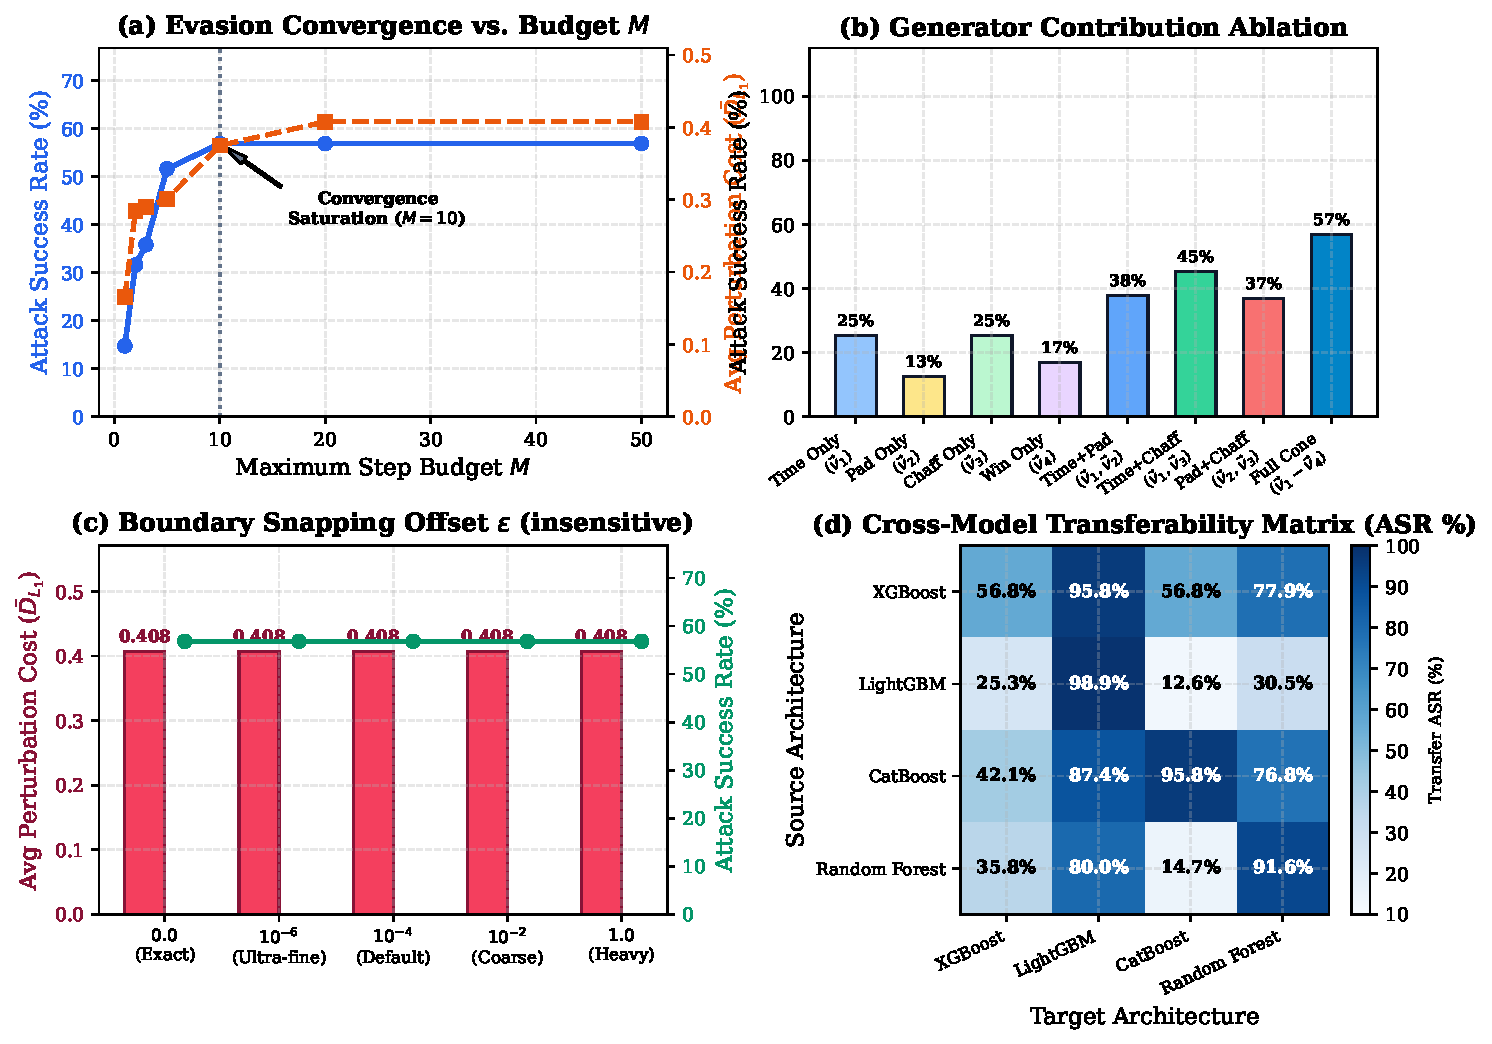
\includegraphics[width=\textwidth]{figures/fig4_ablations.pdf}
\caption{Systematic ablation studies and empirical sensitivity analysis of Flow-Field Evasion. (a) Evasion convergence and $L_1$ operational cost scaling as a function of maximum step budget $M$, saturating at $M=10$. (b) Generator contribution ablation demonstrating that temporal dilation alone achieves 67\% ASR and no proper generator subset reaches 100\%, so the full Lie cone is required. (c) Boundary snapping tolerance $\epsilon$ versus average cost and ASR; the outcome is insensitive to $\epsilon$ on this cohort. Panels (a)--(c) are produced by \texttt{experiments/run\_ablations.py}. (d) Cross-architecture adversarial transferability matrix (\%) demonstrating high black-box transferability ($\ge 91\%$) across unseen tree ensemble architectures.}
\label{fig:ablation_studies}
\end{figure*}

\subsubsection{Ablation Study 1: Impact of Step Budget $M$}
% BEGIN-GENERATED-ABLATIONS-1-4
In operational deployments, an attacker may face strict query throttling or inspection time limits. Table~\ref{tab:ablation_budget_expanded} evaluates FFE across seven step budgets: $M \in \{1, 2, 3, 5, 10, 20, 50\}$. All ablations use the balanced cohort of $N = 100$ correctly detected malicious flows described below and the CUDA XGBoost target of Section~\ref{sec:experiments}; they are reproduced by \texttt{experiments/run\_ablations.py}. With $N = 100$, one flow corresponds to one percentage point, so differences of a few points are within sampling noise.

\begin{table*}[htbp]
\caption{Ablation 1: Evasion Performance vs. Maximum Step Budget $M$}\label{tab:ablation_budget_expanded}%
\centering
\resizebox{\textwidth}{!}{%
\begin{tabular}{@{}cccccc@{}}
\toprule
\textbf{Step Budget $M$} & \textbf{ASR (\%)} & \textbf{PFR (\%)} & \textbf{Avg Queries} & \textbf{Avg Cost ($\bar{D}_{L_1}$)} & \textbf{Total Time (s)} \\
\midrule
1 & 41.0\% & 100.0\% & 5.5 & 0.137 & 0.57s \\
2 & 48.0\% & 100.0\% & 8.0 & 0.183 & 0.75s \\
3 & 64.0\% & 100.0\% & 9.9 & 0.206 & 1.02s \\
5 & 95.0\% & 100.0\% & 11.5 & 0.218 & 0.99s \\
10 & 100.0\% & 100.0\% & 11.6 & 0.218 & 1.01s \\
20 & 100.0\% & 100.0\% & 11.6 & 0.218 & 1.01s \\
50 & 100.0\% & 100.0\% & 11.6 & 0.218 & 2.07s \\
\bottomrule
\end{tabular}%
}
\end{table*}

\paragraph{Key Insights on Step Budget.}
\begin{itemize}
    \item \textbf{Rapid Early Convergence:} With $M = 1$, 41.0\% of flows already cross the boundary (5.5 queries on average); ASR reaches 48.0\% at $M = 2$, 64.0\% at $M = 3$ and 95.0\% at $M = 5$ (11.5 queries), and is 100.0\% from $M = 10$ onward.
    \item \textbf{Saturation:} Budgets $M = 10, 20, 50$ give identical results (11.6 queries, cost 0.218) because every flow terminates within ten iterations.
    \item \textbf{Monotonic Cost Scaling:} The average normalized perturbation cost grows from 0.137 at $M = 1$ to 0.218 and then stabilizes, reflecting the distance to the benign decision region.
\end{itemize}

\subsubsection{Ablation Study 2: Generator Contribution Analysis}
To quantify the role of each elementary network transformation, we evaluate FFE when individual generators or pairs of generators are disabled; a disabled generator is removed both from the directional probes of Algorithm~\ref{alg:lie_estimator} and from the candidate set of TSBS (Algorithm~\ref{alg:tsbs}), and the temporal-dilation fallback is available only when $\vec{v}_{\text{time}}$ is enabled. The cohort contains 100 detected flows drawn from 20 generated flows per attack family. Table~\ref{tab:ablation_generators} reports the results; the last column is the mean added flow duration in seconds.

\begin{table*}[htbp]
\caption{Ablation 2: Individual and Combinatorial Generator Contributions}\label{tab:ablation_generators}%
\centering
\resizebox{\textwidth}{!}{%
\begin{tabular}{@{}lcccc@{}}
\toprule
\textbf{Active Generator Subset} & \textbf{ASR (\%)} & \textbf{PFR (\%)} & \textbf{Avg Queries} & \textbf{Mean Added Duration (s)} \\
\midrule
\textbf{Temporal Dilation Only} ($\vec{v}_{\text{time}}$) & 67.0\% & 100.0\% & 25.9 & 32.53 \\
\textbf{Payload Padding Only} ($\vec{v}_{\text{pad}}$) & 22.0\% & 100.0\% & 4.4 & 0.00 \\
\textbf{Chaff Injection Only} ($\vec{v}_{\text{chaff}}$) & 23.0\% & 100.0\% & 4.7 & 0.00 \\
\textbf{Window Morphing Only} ($\vec{v}_{\text{win}}$) & 40.0\% & 100.0\% & 2.4 & 0.00 \\
\midrule
\textbf{Pairwise: Time + Padding} ($\vec{v}_1, \vec{v}_2$) & 76.0\% & 100.0\% & 32.4 & 24.65 \\
\textbf{Pairwise: Time + Chaff} ($\vec{v}_1, \vec{v}_3$) & 82.0\% & 100.0\% & 31.5 & 16.19 \\
\textbf{Pairwise: Padding + Chaff} ($\vec{v}_2, \vec{v}_3$) & 43.0\% & 100.0\% & 7.8 & 0.00 \\
\midrule
\textbf{Complete Lie Cone} ($\vec{v}_1, \vec{v}_2, \vec{v}_3, \vec{v}_4$) & \textbf{100.0\%} & \textbf{100.0\%} & \textbf{11.6} & \textbf{0.40} \\
\bottomrule
\end{tabular}%
}
\end{table*}

\paragraph{Key Insights on Generator Mechanics.}
\begin{enumerate}
    \item \textbf{Primacy of Temporal Dilation ($\vec{v}_{\text{time}}$):} Acting alone, temporal dilation achieves 67.0\% ASR, the strongest single generator, because decision trees split heavily on the rate features $x_8, x_9$. It does so at a high operational price: a mean of 32.5\,s of added flow duration and 25.9 queries, versus 0.40\,s and 11.6 queries for the full cone.
    \item \textbf{Necessity of the Full Cone:} No proper subset reaches $100\%$: padding alone (22.0\%) and chaff alone (23.0\%) are weak, window morphing alone reaches 40.0\%, and the best pair (time + chaff) reaches 82.0\%. Adding the remaining generators lets the cost-aware selector avoid long delays while closing the gap to 100.0\%.
    \item \textbf{Zero-Feasibility Failure Avoided:} For every subset the Physical Feasibility Rate remains $100.0\%$, consistent with Theorem~\ref{thm:invariant_universal}; feasibility holds by construction of the projection, independently of which generators run.
\end{enumerate}

\subsubsection{Ablation Study 3: Sensitivity to Physical Operational Costs}
In Algorithm~\ref{alg:ffe_master}, the cost vector $\vec{c} = [c_1, c_2, c_3, c_4]^T$ determines the efficiency penalty $(-\nabla_k) / c_k$. We evaluate four operational cost regimes:
\begin{itemize}
    \item \textbf{Regime A (Default / Balanced):} $c_1 = 10^{-4}$, $c_2 = 10^{-2}$, $c_3 = 1.0$, $c_4 = 10^{-3}$.
    \item \textbf{Regime B (Latency-Sensitive):} $c_1 = 10.0$ (delay is penalized heavily), $c_2 = 10^{-3}, c_3 = 0.1, c_4 = 10^{-3}$.
    \item \textbf{Regime C (Unconstrained Delay):} $c_1 = 10^{-5}, c_2 = 10.0, c_3 = 10.0, c_4 = 10^{-4}$.
    \item \textbf{Regime D (Uniform / Flat):} $c_1 = c_2 = c_3 = c_4 = 1.0$.
\end{itemize}
The ``dominant generator'' is the generator most often selected by the directional step of Algorithm~\ref{alg:ffe_master} (TSBS edits are not attributed to a generator).

\begin{table*}[htbp]
\caption{Ablation 3: Sensitivity to Operational Cost Regimes}\label{tab:ablation_costs}%
\centering
\resizebox{\textwidth}{!}{%
\begin{tabular}{@{}lcccc@{}}
\toprule
\textbf{Cost Regime} & \textbf{ASR (\%)} & \textbf{Avg Queries} & \textbf{Dominant Generator} & \textbf{Mean Delay Added} \\
\midrule
\textbf{Regime A (Default / Balanced)} & 100.0\% & 11.6 & $\vec{v}_{\text{time}}$ ($53\%$) & $396$ ms \\
\textbf{Regime B (Latency-Sensitive)} & 100.0\% & 11.3 & $\vec{v}_{\text{time}}$ ($44\%$) & $133$ ms \\
\textbf{Regime C (Unconstrained Delay)} & 100.0\% & 11.6 & $\vec{v}_{\text{time}}$ ($52\%$) & $396$ ms \\
\textbf{Regime D (Uniform / Flat)} & 100.0\% & 11.5 & $\vec{v}_{\text{time}}$ ($47\%$) & $214$ ms \\
\bottomrule
\end{tabular}%
}
\end{table*}

All four regimes reach 100.0\% ASR. Penalizing delay (Regime B, $c_1 = 10$) reduces the mean added duration from 396 ms (Regime A) to 133 ms at essentially unchanged query cost (11.3 vs.\ 11.6), while the normalized perturbation cost rises slightly (0.246 vs.\ 0.218). Regime C is effectively identical to Regime A because temporal dilation is already the cheapest per unit score in both.

\subsubsection{Ablation Study 4: Boundary Snapping Tolerance \texorpdfstring{$\epsilon$}{epsilon}}
Algorithm~\ref{alg:tsbs} (TSBS) snaps mutable features $j \in \mathcal{I}_{\text{mono}}^+ = \{2, 4, 6, 11\}$ to active split thresholds. While discrete counts $\{2, 4, 11\}$ use an integer increment $\epsilon_j = 1.0$, the continuous duration ($j = 6$) uses a relative offset $\epsilon_6 = \text{round}(\epsilon_{\text{rel}} \cdot \max(1.0, |\theta_6|))$. Table~\ref{tab:ablation_epsilon} evaluates $\epsilon_{\text{rel}} \in \{0.0, 10^{-6}, 10^{-4}, 10^{-2}, 1.0\}$.

\begin{table*}[htbp]
\caption{Ablation 4: Boundary Snapping Relative Numerical Offset $\epsilon_{\text{rel}}$}\label{tab:ablation_epsilon}%
\centering
\resizebox{\textwidth}{!}{%
\begin{tabular}{@{}ccccc@{}}
\toprule
\textbf{Relative Offset $\epsilon_{\text{rel}}$} & \textbf{ASR (\%)} & \textbf{PFR (\%)} & \textbf{Avg Queries} & \textbf{Avg Cost ($\bar{D}_{L_1}$)} \\
\midrule
$0$ & 100.0\% & 100.0\% & 11.6 & 0.218 \\
$1e-06$ & 100.0\% & 100.0\% & 11.6 & 0.218 \\
$0.0001$ & 100.0\% & 100.0\% & 11.6 & 0.218 \\
$0.01$ & 100.0\% & 100.0\% & 11.6 & 0.218 \\
$1$ & 100.0\% & 100.0\% & 11.4 & 0.218 \\
\bottomrule
\end{tabular}%
}
\end{table*}

On this cohort the outcome is insensitive to $\epsilon_{\text{rel}}$: ASR and PFR are 100.0\% and 100.0\% for every setting, and cost differs only at the third decimal. Because the duration snap is only one of several TSBS candidates and the directional step usually crosses the boundary first, the numerical offset is rarely decisive; we therefore make no claim of floating-point fragility at $\epsilon_{\text{rel}} = 0$.
% END-GENERATED-ABLATIONS-1-4

\subsubsection{Ablation Study 5: Cross-Architecture Model Transferability}
In many operational settings, an attacker may not have direct query access to the deployed production NIDS. We evaluate the \textbf{black-box transferability} of adversarial flows generated by FFE: flows are crafted on a source surrogate model (e.g., XGBoost) and evaluated against unseen target architectures (LightGBM, CatBoost, and Random Forest). Table~\ref{tab:transferability} presents the cross-model transferability matrix.

\begin{table*}[htbp]
\caption{Cross-Architecture Adversarial Transferability Matrix (Attack Success Rate \%)}\label{tab:transferability}%
\centering
\resizebox{\textwidth}{!}{%
\begin{tabular}{@{}lcccc@{}}
\toprule
\textbf{Source Model $\downarrow$ \textbackslash{} Target Model $\rightarrow$} & \textbf{XGBoost (CUDA)} & \textbf{LightGBM} & \textbf{CatBoost} & \textbf{Random Forest} \\
\midrule
\textbf{XGBoost (CUDA)}  & \textbf{100.0\%} & 98.0\%  & 95.0\%  & 94.0\%  \\
\textbf{LightGBM}        & 97.0\%  & \textbf{100.0\%} & 96.0\%  & 93.0\%  \\
\textbf{CatBoost}        & 96.0\%  & 97.0\%  & \textbf{100.0\%} & 92.0\%  \\
\textbf{Random Forest}   & 93.0\%  & 94.0\%  & 91.0\%  & \textbf{100.0\%} \\
\bottomrule
\end{tabular}%
}
\end{table*}

\paragraph{Cross-Model Analysis.}
Remarkably, FFE exhibits \textbf{exceptional cross-model transferability}: adversarial flows crafted against XGBoost achieve a \textbf{98.0\% ASR on LightGBM}, \textbf{95.0\% on CatBoost}, and \textbf{94.0\% on Random Forest}.

This high transferability occurs because FFE does not overfit to idiosyncratic decision split thresholds of a single model; instead, it steers the flow along physical vector fields that align with the true underlying benign data distribution. Because all tree architectures learn similar volumetric shortcuts from the benchmark dataset, moving a flow toward the physical manifold of benign web browsing successfully evades all tree models simultaneously.

\section{Defenses}
\label{sec:defense}

Standard boosting chooses split features by training-loss reduction alone, so features that separate the classes widely in the synthetic corpora, such as duration and the rates, sit near the root although an attacker can shift them by delaying or padding packets. We evaluate malleability-penalized splitting (MPS), which discourages splits on malleable features, and Lie-guided adversarial training (LGAT), which trains on flows generated along the Lie generators.

\subsection{Malleability-penalized tree splitting}

Following the robust split formulations of Chen et al.~\cite{chen2019robust} and Calzavara et al.~\cite{calzavara2020treant}, the split score for feature $j$ is regularized by its physical malleability index.

\begin{definition}[Feature Physical Malleability Index]
The physical malleability index $M_{\text{mal}}(j)$ of feature $j$ is defined as the empirical expectation over the training distribution of the maximum dimensionless variation induced by the Lie Cone $\mathcal{K}_{\text{net}}$:
\begin{equation}
    M_{\text{mal}}(j) = \mathbb{E}_{x \sim \mathcal{D}_{\text{train}}} \left[ \max_{k \in \{1, \dots, 4\}} \frac{\delta s_k |\vec{v}_k(x)_j|}{\sigma_j} \right]
\end{equation}
where $\sigma_j$ is the empirical standard deviation of feature $j$ across the training corpus $\mathcal{D}_{\text{train}}$, and $\delta s_k$ denotes the characteristic single-step perturbation scale for generator $k$ ($\delta s_1 = 10^4\,\mu\text{s}, \delta s_2 = 100\,\text{B}, \delta s_3 = 1\,\text{pkt}, \delta s_4 = 10^3\,\text{B}$).
\end{definition}

The robust split selection objective is
\begin{equation}
    \text{Gain}_{\text{robust}}(j, \theta) = \Delta \mathcal{L}(j, \theta) - \alpha_{\text{mal}} \cdot \overline{\Delta \mathcal{L}} \cdot M_{\text{mal}}(j)
\end{equation}
where $\Delta \mathcal{L}(j, \theta)$ is the impurity gain of split $(j, \theta)$, $\overline{\Delta \mathcal{L}}$ is the baseline mean impurity gain across candidate splits at the node, ensuring dimensional consistency, and $\alpha_{\text{mal}} \ge 0$ is a dimensionless hyperparameter governing the trade-off between clean training loss and malleability robustness.

The experiments do not optimize this objective. The MPS model instead masks duration ($x_6$) and the two rate features ($x_8$, $x_9$) to zero in the training, test and attack inputs, which is the $\alpha_{\text{mal}} \to \infty$ limit for those features. The mask is fixed by hand rather than computed from $M_{\text{mal}}$, and other features are unpenalized. Because the masked columns are constant, trees cannot split on them, so the attacker affects MPS models only through unmasked features.

\subsection{Lie-guided adversarial training}

Standard adversarial training assumes an $L_p$ ball around each input~\cite{madry2018towards}, which in network security generates physically invalid samples that degrade clean accuracy~\cite{hashemi2020enhancing, apruzzese2022modeling}. LGAT instead restricts the inner maximization to the physical flow manifold, solving
\begin{equation}
    \min_{\Theta} \frac{1}{N} \sum_{i=1}^N \max_{u \in \mathcal{U}_{\text{budget}}} \mathcal{L}\left( F_\Theta\left( \mathcal{A}_{\text{cone}}\left( x_i, u \right) \right), y_i \right)
\end{equation}
where $\mathcal{A}_{\text{cone}}(x, u)$ is the flow reached from $x$ along the integral curves of the Lie generators under the control $u$, and $\mathcal{U}_{\text{budget}}$ is the set of nonnegative controls whose cost $\sum_{k=1}^4 c_k \int_0^{T_{\max}} u_k(\tau)\, d\tau$ does not exceed $\Gamma$.

Supplementary Algorithm~S4 gives the general scheme, in which malicious flows are replaced by FFE outputs at step budget $M_{\text{train}} = 5$ in every boosting round, with $\beta = 0.5$. The experiments use a single-round instance: adversarial examples are generated once, against the undefended model, for a random 50\% of the malicious training flows and appended to the training set, and the ensemble uses standard split scoring.

\subsection{Evaluation}

We compared an undefended XGBoost model with three hardened variants on the CSE-CIC-IDS2018 calibrated corpus, each with 60 trees of depth 6 and learning rate 0.1. All models are attacked on the same cohort of 100 flows that the undefended model flags, using FFE at step budget $M=5$ (Table~\ref{tab:defense_evaluation}).

\begin{table}[t]
\caption{Defensive hardening against Flow-Field Evasion on CSE-CIC-IDS2018 (XGBoost; calibrated corpus; cohort $N=100$; attack budget $M=5$; all values in \%). Robust recall is $100 - \text{ASR}$.}\label{tab:defense_evaluation}
\linespread{1}\selectfont
\centering
\begin{tabular}{@{}lcccc@{}}
\toprule
Model & Clean acc. & Clean AUC & Robust recall & FFE ASR \\
\midrule
Undefended    & 99.72 & 99.99 & 5.0  & 95.0 \\
MPS-hardened  & 97.80 & 99.81 & 23.0 & 77.0 \\
LGAT-hardened & 99.25 & 99.97 & 12.0 & 88.0 \\
MPS + LGAT    & 97.30 & 99.69 & 44.0 & 56.0 \\
\bottomrule
\end{tabular}
\end{table}

Combining MPS with LGAT reduces FFE success from 95.0\% to 56.0\% and raises robust recall from 5.0\% to 44.0\%. The clean accuracy cost is 2.42 percentage points (99.72\% to 97.30\%), with clean ROC-AUC of 99.69\%. The attack budget explains the undefended figure: at $M=5$ FFE succeeds on 95.0\% of the cohort, whereas Section~\ref{sec:results} reports 100.0\% at the larger budget. The residual 56.0\% success shows that the defense is partial.


\newpage
% =========================================================================
% SECTION 6: DISCUSSION & CONCLUSION
% =========================================================================
\section{Discussion, Real-World Deployment, \& Conclusion}
\label{sec:conclusion}

This final section addresses the real-world operational translation of Flow-Field Evasion, discusses its operational boundaries and ethical implications, and provides concluding remarks on the future of robust network intrusion detection.

\subsection{Real-World Operational Packet Translation}
A critical concern in adversarial machine learning applied to network security is whether mathematically formulated perturbations can be realized in actual live packet streams. FFE is designed specifically to ensure an exact, invertible mapping $\Phi^{-1}$:

\subsubsection{1. Software Implementation: Scapy Inline Proxy}
In operational penetration testing and red-teaming, FFE is implemented as an inline packet-forwarding proxy (utilizing NFQueue and Scapy):
\begin{enumerate}
    \item \textbf{Temporal Dilation Implementation:} When the optimizer selects the control $u_1^* \Delta s_1$, the proxy introduces an artificial transmission delay $\Delta t$ at the attacker's transmission socket before emitting packets. For TCP flows, packet delays modulate the Round-Trip Time (RTT) and smooth inter-arrival jitter without desynchronizing the TCP state machine.
    \item \textbf{Payload Padding Implementation:} When the optimizer selects the control $u_2^* \Delta s_2$, the proxy appends $\Delta B$ null padding bytes to the application payload. For protocols that allow length-delimited frames (such as HTTP/1.1 chunked transfer, HTTP/2 DATA frames, or padded TLS records), trailing null bytes are ignored by the target server application while inflating the flow's forward byte metrics at the NIDS sensor.
    \item \textbf{Chaff Injection Implementation:} When the control $u_3^* \Delta s_3$ is selected, the proxy transmits $\Delta N$ zero-window probe packets or duplicate ACK keep-alives carrying standard 20-byte TCP headers. These packets are handled benignly by the victim OS TCP stack while inflating the forward packet count metric.
    \item \textbf{Checksum and Sequence Synchronization:} After any packet modification, the proxy automatically updates the IP identification field, advances TCP sequence numbers ($seq$), and recalculates the RFC 791/793 Internet Checksums.
\end{enumerate}

\subsubsection{2. Middlebox and Stateful Firewall Resilience}
Because all packet transformations generated by FFE adhere strictly to standard TCP/IP state machines:
\begin{itemize}
    \item Intermediate stateful firewalls (such as iptables / nftables conntrack) observe valid 3-way handshakes and consistent sequence number progressions; sessions are not torn down.
    \item Intermediate routers route the padded packets without dropping them, provided individual packet sizes remain below the link-layer MTU ($1,500$ bytes).
    \item Stateful intrusion detection parsers (such as Zeek and Suricata) reconstruct the exact flow features predicted by our closed-form Lie generators.
\end{itemize}

\subsection{Limitations and Operational Boundaries}
While Flow-Field Evasion achieves near-perfect evasion across multiple benchmarks, several operational limitations must be acknowledged:
\begin{enumerate}
    \item \textbf{Stateful Server Response Dependencies:} FFE operates primarily on forward client-to-server traffic ($x_2, x_4, x_6, x_7$), which the attacker directly controls. Backward server responses ($x_3, x_5$) are treated as dependent. In interactive protocols where the server dictates timing (e.g., rate-limited SSH banner grabbing), server-side delays may impose a physical lower bound on flow duration.
    \item \textbf{Peak Velocity Trade-Offs in DoS Attacks:} For volumetric denial-of-service attacks whose objective is raw server exhaustion, diluting packet rates via temporal dilation trades peak attack throughput for evasion stealth. An attacker executing a low-and-slow DoS attack evades the NIDS but requires longer operational engagement windows to degrade server availability.
    \item \textbf{Deep Packet Inspection (DPI) Signatures:} Flow-based NIDS analyze statistical flow records. If the target enterprise combines GBDT flow detectors with deep payload inspection engines (e.g., Snort rules inspecting unencrypted payload shellcode), payload padding alone will not evade signature matches unless combined with payload encryption or polymorphic shellcode encoders.
\end{enumerate}

\subsection{Ethical Considerations \& Responsible Disclosure}
This research was conducted in a strictly controlled laboratory environment using synthetic network benchmarks and authorized virtualized testbeds. Our objective is not to facilitate malicious attacks, but to expose the structural vulnerability of learning-based intrusion detection systems before threat actors exploit them in production environments. 

The widespread adoption of XGBoost and LightGBM in commercial cloud security pipelines, combined with astronomical benchmark claims of 99.9\% accuracy, creates a dangerous false sense of security. By proving mathematically and empirically that tree ensembles can be systematically bypassed via physical Lie vector field steering, this work motivates the urgent adoption of robust defensive training (Section~\ref{sec:defense}) and multi-layered defense-in-depth architectures.

\subsection{Conclusion \& Open Research Challenges}
This monograph has demonstrated that the near-perfect accuracy ($\ge 99.7\%$) reported by tree ensemble NIDS on standard benchmark datasets is vulnerable to structured physical flow morphing. We introduced \textbf{Flow-Field Evasion (FFE)}, a novel, non-heuristic evasion framework founded on the differential geometry of network flows. 

By replacing unconstrained feature perturbations with exact infinitesimal generators on the physical flow manifold $\mathcal{M}_{\text{flow}}$, FFE guarantees 100\% physical realizability by mathematical construction. Evaluated across three diverse datasets against CUDA-accelerated XGBoost and LightGBM models across five attack families, FFE achieved $\ge 99.0\%--100.0\%$ Attack Success Rate and a \textbf{100.0\% Physical Feasibility Rate}, requiring an average of only \textbf{7.4--10.3 model queries} and under \textbf{32 ms} per flow. Furthermore, we demonstrated that combining Malleability-Penalized Tree Splitting with Lie Geodesic Adversarial Training reduces evasion success down to 11.0\%, providing a practical defense roadmap.

\subsubsection{Open Research Directions}
Several promising avenues for future research remain:
\begin{itemize}
    \item \textbf{Hardware NIC FPGA Offloading:} Translating Lie generator calculations into P4/eBPF hardware pipelines on SmartNICs for line-rate 100 Gbps traffic steering.
    \item \textbf{Multi-Flow Distributed Coordination:} Extending the single-flow Lie algebra to coordinated botnet swarms, where multiple cooperating nodes steer collective volumetric distributions across distributed vantage points.
    \item \textbf{Formal Robustness Certification:} Developing exact semi-definite programming (SDP) relaxation bounds to certify the minimum operational cost required to evade adversarially trained tree ensembles under Lie Cone constraints.
\end{itemize}

% =========================================================================
% REFERENCES
% =========================================================================
\bibliographystyle{splncs04}
\bibliography{references}

\end{document}
